%%%%%%%%%%%%%%%%%%%%%%%%%%%%%%%%%%%%%%%%%
% Masters/Doctoral Thesis 
% LaTeX Template
% Version 2.4 (22/11/16)
%
% This template has been downloaded from:
% http://www.LaTeXTemplates.com
%
% Version 2.x major modifications by:
% Vel (vel@latextemplates.com)
%
% This template is based on a template by:
% Steve Gunn (http://users.ecs.soton.ac.uk/srg/softwaretools/document/templates/)
% Sunil Patel (http://www.sunilpatel.co.uk/thesis-template/)
%
% Template license:
% CC BY-NC-SA 3.0 (http://creativecommons.org/licenses/by-nc-sa/3.0/)
%
%%%%%%%%%%%%%%%%%%%%%%%%%%%%%%%%%%%%%%%%%

%----------------------------------------------------------------------------------------
%	PACKAGES AND OTHER DOCUMENT CONFIGURATIONS
%----------------------------------------------------------------------------------------

\documentclass[
11pt, % The default document font size, options: 10pt, 11pt, 12pt
oneside, % Two side (alternating margins) for binding by default, uncomment to switch to one side
english, ukrainian, % ngerman for German
singlespacing, % Single line spacing, alternatives: onehalfspacing or doublespacing
%draft, % Uncomment to enable draft mode (no pictures, no links, overfull hboxes indicated)
%nolistspacing, % If the document is onehalfspacing or doublespacing, uncomment this to set spacing in lists to single
%liststotoc, % Uncomment to add the list of figures/tables/etc to the table of contents
%toctotoc, % Uncomment to add the main table of contents to the table of contents
parskip, % Uncomment to add space between paragraphs
%nohyperref, % Uncomment to not load the hyperref package
headsepline, % Uncomment to get a line under the header
%chapterinoneline, % Uncomment to place the chapter title next to the number on one line
%consistentlayout, % Uncomment to change the layout of the declaration, abstract and acknowledgements pages to match the default layout
]{MastersDoctoralThesis} % The class file specifying the document structure

\usepackage[utf8]{inputenc} % Required for inputting international characters
\usepackage[T2A, T1]{fontenc} % Output font encoding for international characters


\usepackage{palatino} % Use the Palatino font by default

%\usepackage[backend=bibtex,style=authoryear,natbib=true]{biblatex} % Use the bibtex backend with the authoryear citation style (which resembles APA)
\usepackage[backend=bibtex,sorting=none,natbib=true]{biblatex}
%\usepackage{natbib}

\addbibresource{example.bib} % The filename of the bibliography

\usepackage[ruled,vlined]{algorithm2e}
\usepackage{amsthm}
\usepackage{amssymb}
\usepackage{graphicx}
\usepackage{amsmath}
\usepackage{amssymb}
\usepackage{enumitem}
\usepackage[nottoc,numbib]{tocbibind}
\usepackage{multirow}
\usepackage{hyperref}


%\usepackage[autostyle=true]{csquotes} % Required to generate language-dependent quotes in the bibliography


%----------------------------------------------------------------------------------------
%	MARGIN SETTINGS
%----------------------------------------------------------------------------------------

\geometry{
	paper=a4paper, % Change to letterpaper for US letter
	inner=2.5cm, % Inner margin
	outer=2.5cm, % Outer margin
	bindingoffset=.5cm, % Binding offset
	top=1.5cm, % Top margin
	bottom=1.5cm, % Bottom margin
	%showframe, % Uncomment to show how the type block is set on the page
}

%----------------------------------------------------------------------------------------
%	THESIS INFORMATION
%----------------------------------------------------------------------------------------

\thesistitle{Thesis Title} % Your thesis title, this is used in the title and abstract, print it elsewhere with \ttitle
\supervisor{Dr. James \textsc{Smith}} % Your supervisor's name, this is used in the title page, print it elsewhere with \supname
\examiner{} % Your examiner's name, this is not currently used anywhere in the template, print it elsewhere with \examname
\degree{Doctor of Philosophy} % Your degree name, this is used in the title page and abstract, print it elsewhere with \degreename
\author{John \textsc{Smith}} % Your name, this is used in the title page and abstract, print it elsewhere with \authorname
\addresses{} % Your address, this is not currently used anywhere in the template, print it elsewhere with \addressname

\subject{Biological Sciences} % Your subject area, this is not currently used anywhere in the template, print it elsewhere with \subjectname
\keywords{} % Keywords for your thesis, this is not currently used anywhere in the template, print it elsewhere with \keywordnames
\university{\href{http://www.univ.kiev.ua/}{Київський національний університет імені Тараса Шевченка}} % Your university's name and URL, this is used in the title page and abstract, print it elsewhere with \univname
\department{\href{http://om.univ.kiev.ua/}{кафедри обчислювальної математики}} % Your department's name and URL, this is used in the title page and abstract, print it elsewhere with \deptname
\group{\href{http://researchgroup.university.com}{Research Group Name}} % Your research group's name and URL, this is used in the title page, print it elsewhere with \groupname
\faculty{\href{http://cyb.univ.kiev.ua/}{факультет комп'ютерних наук та кібернетики}} % Your faculty's name and URL, this is used in the title page and abstract, print it elsewhere with \facname

\AtBeginDocument{
\hypersetup{pdftitle=\ttitle} % Set the PDF's title to your title
\hypersetup{pdfauthor=\authorname} % Set the PDF's author to your name
\hypersetup{pdfkeywords=\keywordnames} % Set the PDF's keywords to your keywords
}

\begin{document}

\frontmatter % Use roman page numbering style (i, ii, iii, iv...) for the pre-content pages

\pagestyle{plain} % Default to the plain heading style until the thesis style is called for the body content

%----------------------------------------------------------------------------------------
%	TITLE PAGE
%----------------------------------------------------------------------------------------

\begin{titlepage}
	\centering
	{\scshape\Large\univname\par}
	{\scshape\Large\facname\par} 
	\vspace{3cm}
	
	{\Large\bfseries Випускна кваліфікаційна робота бакалавра\par}
	{\Large на тему:\par}
	{\LARGE \enquote{Розпізнавання раку молочної залози за допомогою аналізу інтерфазних ядер букального епітелію} \par}
	\vspace{3cm}
	
	\flushright
	{\large Студента 4 курсу \par}
	{\large \deptname \par}	
	{\large \href{tranhavu@knu.ua}{Чан Ха Ву}\par}
	\vspace{1cm}
	
	{\large Науковий керівник \par}
	{\large професор, доктор фізико-математичних наук\par}
	{\large \href{dokmed5@gmail.com}{Клюшин Дмитро Анатолійович}\par}
	\vspace{2cm}
	
	\flushleft	
	{\large Робота заслухана на засіданні кафедри обчислювальної математики та рекомендована до захисту в ДЕК, протокол № 11 від 18 травня 2017 р.\par}
	\vspace{1cm}
	{\large Завідувач кафедри обчислювальної математики \hfill проф. Ляшко С.І.\par}
	\vspace{1cm}
	
	\centering
	\vfill
	{\large Київ}
	{\large 2017} 
\end{titlepage}


% Ukrainization and some other customizations
\newenvironment{megaalgorithm}[1][htb]
{\renewcommand{\algorithmcfname}{Алгоритм}% Update algorithm name
	\begin{algorithm}[#1]%
	}{\end{algorithm}}

\renewcommand{\contentsname}{Зміcт}
\renewcommand{\figurename}{Мал.}
\renewcommand{\refname}{Список літератури}

\theoremstyle{plain}
\newtheorem{thm}{Теорема}
\newtheorem{lem}[thm]{Lemma}
\newtheorem{prop}[thm]{Proposition}
\newtheorem*{cor}{Corollary}

\theoremstyle{plain}
\newtheorem{defn}{Означення}
\newtheorem{conj}{Припущення}
\newtheorem{exmp}{Example}

\theoremstyle{remark}
\newtheorem*{rem}{Remark}
\newtheorem*{note}{Note}


%----------------------------------------------------------------------------------------
%	ABSTRACT PAGE
%----------------------------------------------------------------------------------------

\begin{abstract}
\addchaptertocentry{\abstractname} % Add the abstract to the table of contents

У зв'язку зі стрімким зростанням кількості випадків захворювань раком молочної залози, проблема неінвазивної діагностики цієї хвороби є дуже актуальною. Новітні дослід- ження в області онкології \citep{bib:the_beginning} виявили закономірність, яка полягає в тому, що їснує зв'язок між змінами у інтерфазному ядрі букального епітелію та розвитком злоякісної або доброякісної пухлини (раком молочної залози та фіброаденоматозом відповідно). В роботі досліджується цей зв'язок за допомогою технік комп'ютерного зору, фрактальної геометрії та машинного навчання.

Ця робота складається з трьох частин. У першій частині пропонується алгоритм сегмен- тації інтерфазних ядер букального епітелію на зображенні. У другій частині використо- вується фрактальний аналіз інтерфазних ядер букального епітелію, щоб відрізнити здо- рових пацієнтів від хворих раком молочної залози або фіброаденоматозом. У третій частині використовуються методи глибинного навчання для класифікації зразків (зобра- жень) на групи хворих раком молочної залози та хворих фіброаденоматозом.

\end{abstract}

%----------------------------------------------------------------------------------------
%	ACKNOWLEDGEMENTS
%----------------------------------------------------------------------------------------

\begin{acknowledgements}
\addchaptertocentry{Подяка} % Add the acknowledgements to the table of contents

\begin{center}{\huge\textit{Подяки}\par}\end{center}
%The acknowledgments and the people to thank go here, don't forget to include your project advisor\ldots

Хочу виразити щиру подяку своєму науковому керівнику, професору та доктору ф-м наук Клюшину Дмитрові Анатолійовичу, хто надав мені можливість займатися цим неймовірно цікавим дослідженням.

Моїй матері, яка успішно переборола рак молочної залози у 2011-му році та завжди мене підтримувала в навчанні.

Та Анні Разумовій, що допомогла мені в оформленні тексту цієї роботи.

\end{acknowledgements}

%----------------------------------------------------------------------------------------
%	LIST OF CONTENTS/FIGURES/TABLES PAGES
%----------------------------------------------------------------------------------------

\tableofcontents % Prints the main table of contents

%\listoffigures % Prints the list of figures

%\listoftables % Prints the list of tables

%----------------------------------------------------------------------------------------
%	ABBREVIATIONS
%----------------------------------------------------------------------------------------

%\begin{abbreviations}{ll} % Include a list of abbreviations (a table of two columns)

%\textbf{LAH} & \textbf{L}ist %\textbf{A}bbreviations \textbf{H}ere\\
%\textbf{WSF} & \textbf{W}hat (it) \textbf{S}tands \textbf{F}or\\

%\end{abbreviations}

%----------------------------------------------------------------------------------------
%	SYMBOLS
%----------------------------------------------------------------------------------------

%\begin{symbols}{lll} % Include a list of Symbols (a three column table)

%$a$ & distance & \si{\meter} \\
%$P$ & power & \si{\watt} (\si{\joule\per\second}) \\
%Symbol & Name & Unit \\

%\addlinespace % Gap to separate the Roman symbols from the Greek

%$\omega$ & angular frequency & \si{\radian} \\

%\end{symbols}


%----------------------------------------------------------------------------------------
%	THESIS CONTENT - CHAPTERS
%----------------------------------------------------------------------------------------

\mainmatter % Begin numeric (1,2,3...) page numbering

\pagestyle{thesis} % Return the page headers back to the "thesis" style

% Include the chapters of the thesis as separate files from the Chapters folder
% Uncomment the lines as you write the chapters

% Chapter Template

\chapter{Вступ} % Main chapter title

\label{Chapter1} % Change X to a consecutive number; for referencing this chapter elsewhere, use \ref{ChapterX}

Незважаючи на стрімкий розвиток сучасної онкології, захворюваність на рак молочної залози як в Україні, так і в більшості розвинених країн світу продовжує зростати. Щороку у світі реєструють більше п’яти тисяч нових випадків захворювання на рак молочної залози, що становить понад 25\% всіх ракових захворювань у жінок. Тому задача неінвазивної діагностики раку молочної залози є надзвичайно актуальною.

Обробка цифрових зображень давно стала складовою досліджень практично у всіх галу- зях науки. Робота зі зразками з будь-якої предметної області має на увазі не тільки витяг даних із зображень, але і класифікацію знімків, роботу зі складноструктурованими зразками, з неочевидними закономірностями і особливостями, часто помітними лише фахівцям у цій галузі. У медицині можливість автоматично обробляти та розпізнавати великі набори знімків мікроскопа певної тематики може значно вплинути на хід дослід- жень, полегшити процес роботи із зображеннями та у результаті, наприклад, прискорити виявлення хвороби та постановку діагнозу, що допоможе підібрати своєчасне і необхідне лікування.


\section{Метод дослідження}

Як показано у попередніх роботах в області онкології \citep{bib:the_beginning}, злоякісні та доброякісні утво- рення певним чином впливають на інтерфазні ядра букального епітелію. Ми сподіваємось що використовуючи методи комп'ютерного зору, фрактального аналізу та машинного навчання, можна діагнозувати рак молочної залози та фіброаденоматоз (доброякісна пухлина) з певною точністю.

\section{Опис даних}

Для дослідження було використано набір зображень інтерфазних ядер букального епі- телію, отриманих від здорових пацієнтів, а також хворих раком молочної залози та фіброаденоматозом, які лікувались у інституті онкології. Вхідний набір даних для скла- дається з знімків 6752 інтерфазних ядер букального епітелію, для кожного було зроблено 3 знімки мікроскопу (сканограми оптичної щільності): без фільтру, через жовтий фільтр та через пурпурного фільтру (отже всьго 20256 фотографії), взятого з 130 пацієнтів, з них 68 хворих раком, 29 здорових та 33 хворих фіброаденоматозом. 

% Chapter Template

\chapter{Попередня обробка даних} % Main chapter title

\label{Chapter2} % Change X to a consecutive number; for referencing this chapter elsewhere, use \ref{ChapterX}

%----------------------------------------------------------------------------------------
%	SECTION 1
%----------------------------------------------------------------------------------------

\section{Сегментація ядер}

\begin{figure}[b!]
	\minipage{0.333\textwidth}
	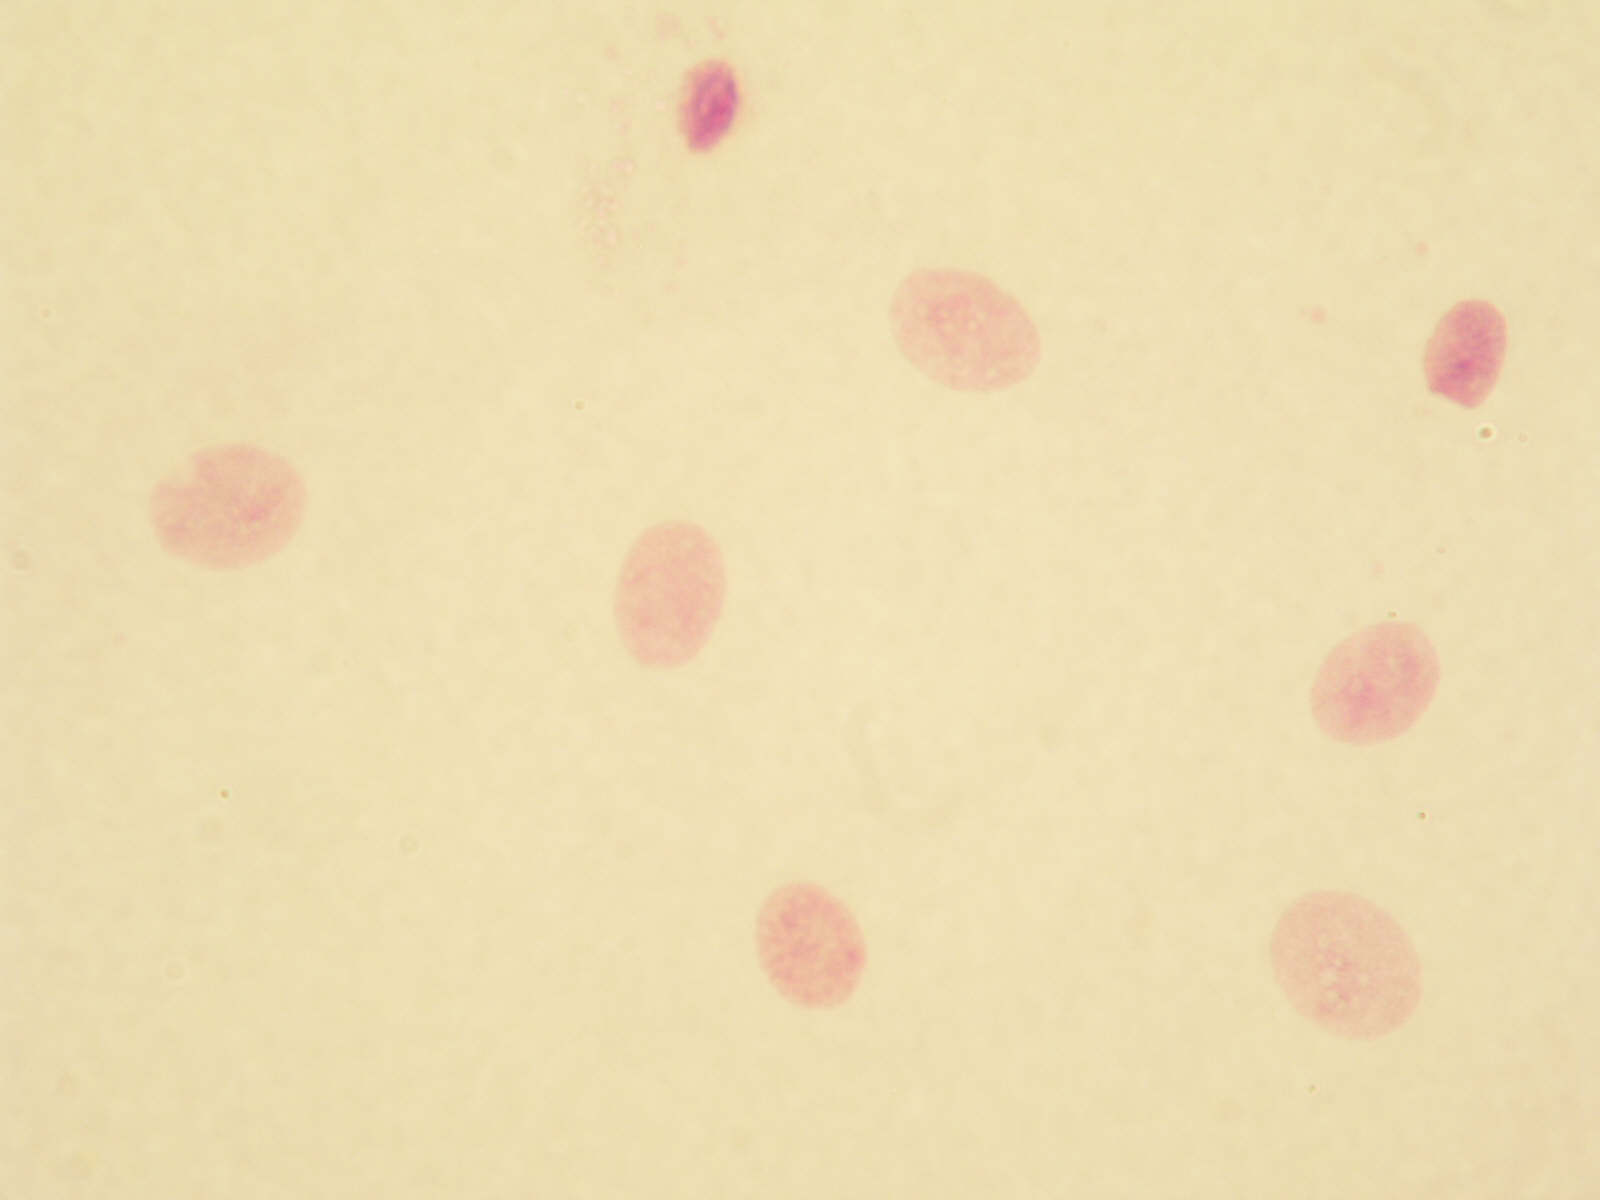
\includegraphics[width=0.97\linewidth]{Figures/Chapter2/0a.png}
	\centering
	\endminipage\hfill
	\minipage{0.333\textwidth}
	\centering	
	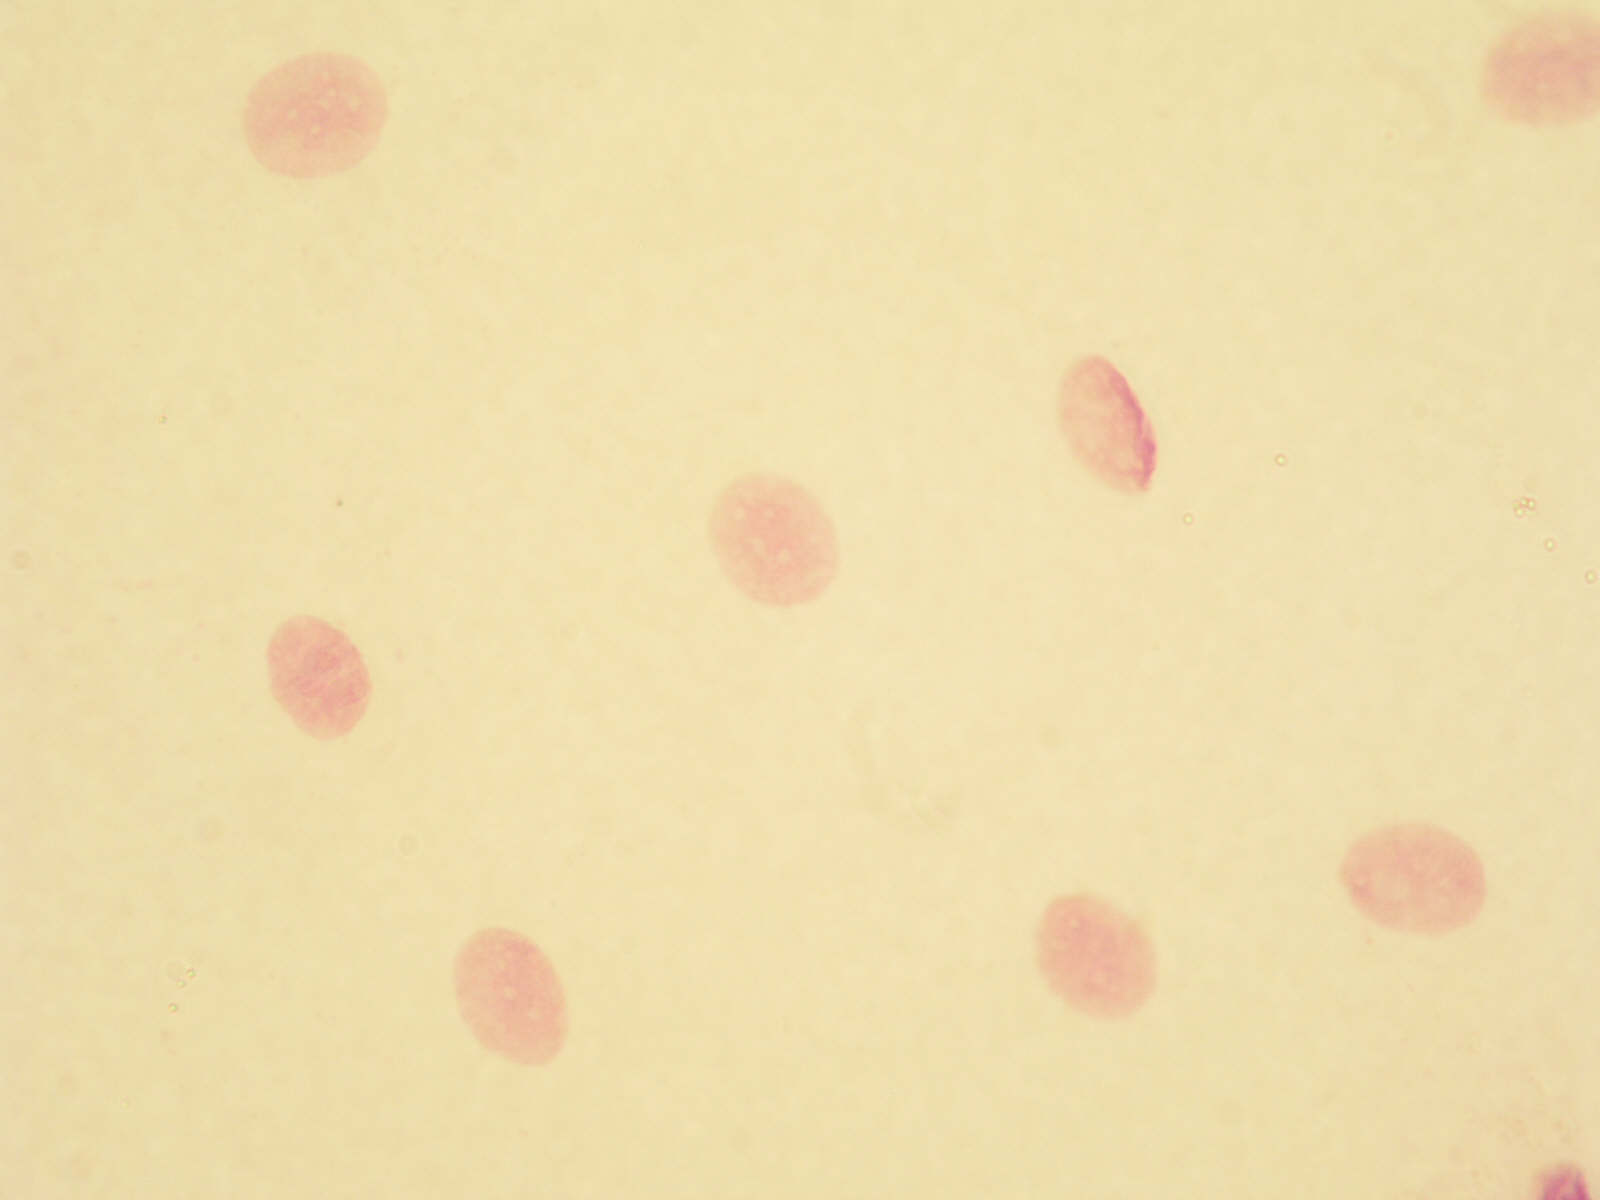
\includegraphics[width=0.97\linewidth]{Figures/Chapter2/0b.png}
	\endminipage\hfill
	\minipage{0.333\textwidth}
	\centering	
	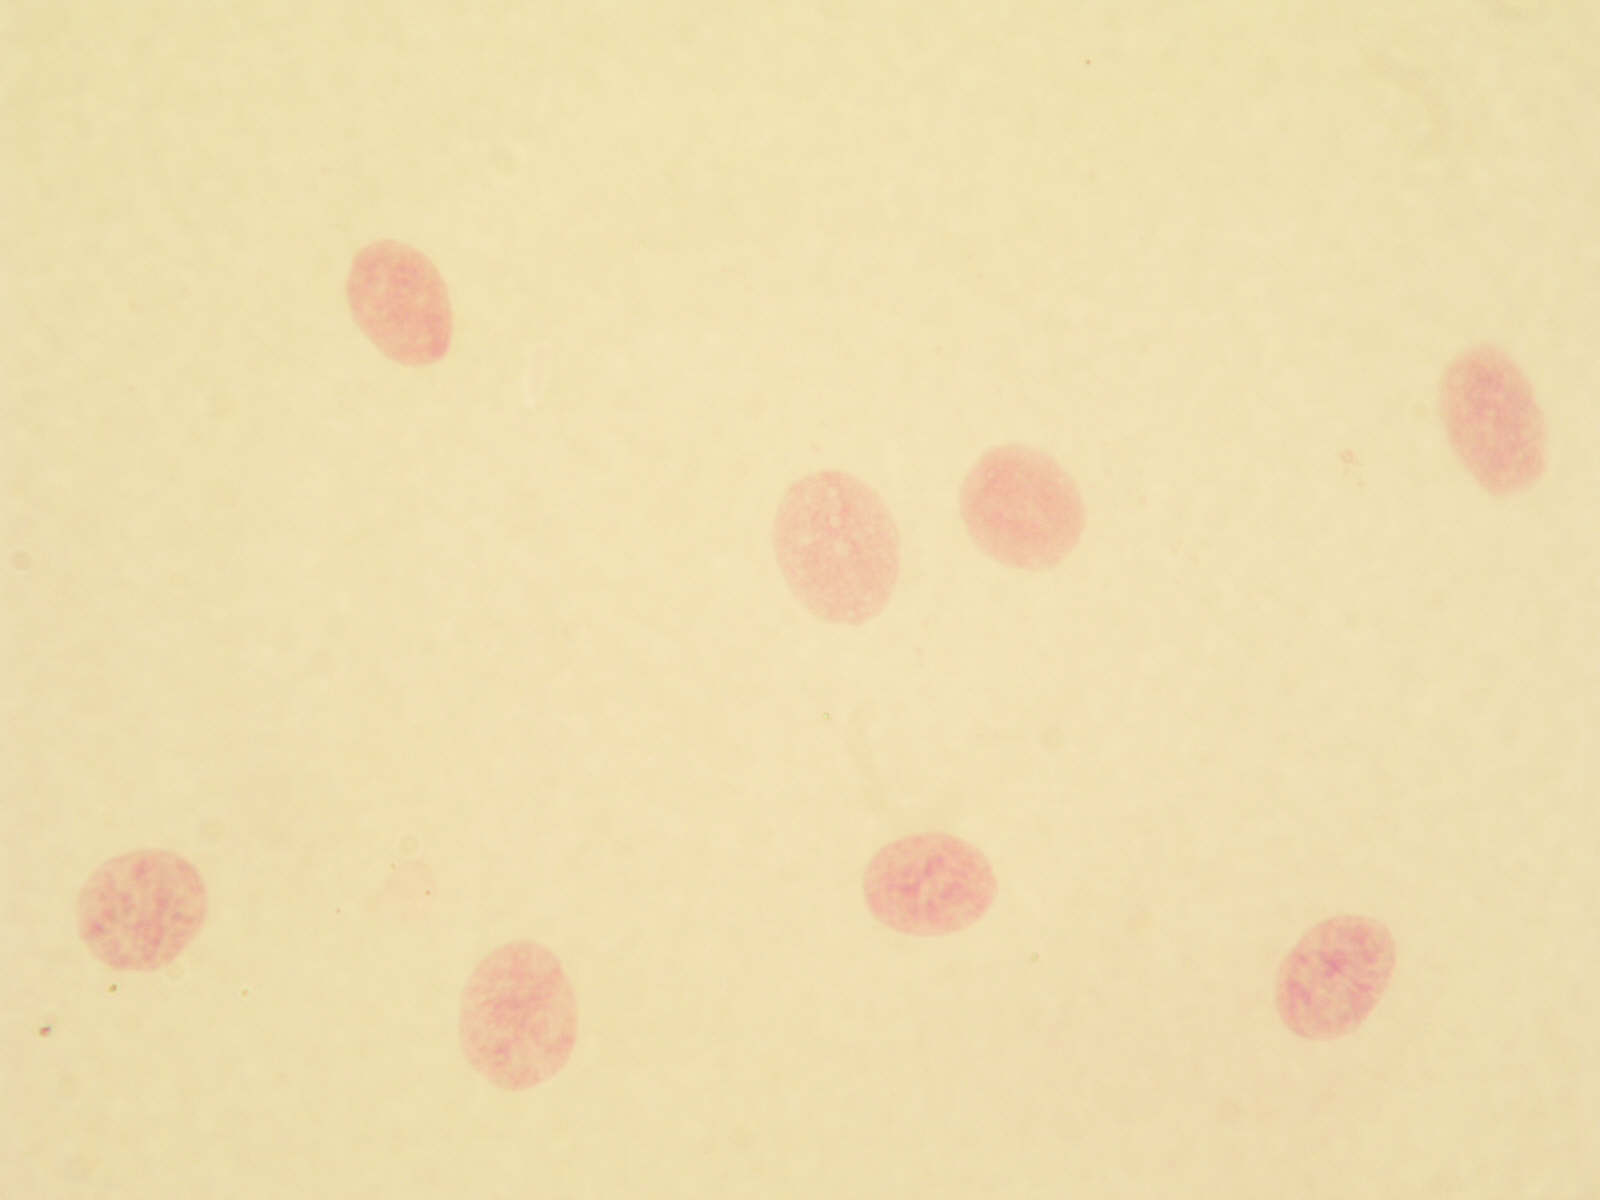
\includegraphics[width=0.97\linewidth]{Figures/Chapter2/0c.png}
	\endminipage\hfill
	
	\caption{Зображення інтерфазних ядер букального епітелію, які треба сегментувати.}
	\label{fig:raw_cells}
\end{figure}

\par
Мікроскопічні зображення у чистому вигляді зазвичай неприйнятні для аналізу у зв’язку з наявністю дефектів, цифрових шумів, спричинених необхідністю підвищення світло- чутливості фотоматеріалів, а також сторонніх об’єктів. Отже, для подальшого аналізу вхідного набору зображень (або набору пацієнтів), необхідно зробити попередню обробку та сегментацію.

\par
На (Мал.~\ref{fig:raw_cells}) зображено приклади знімків інтерфазних ядер букального епітелію. З них треба виділити окремі клітини для подальшого аналізу. Задача обробки та сегментації зображень розбивається на наступні підзадачі:

\begin{enumerate}
	\item Зменшення шуму
	\item Відділення фону
	\item Виділення окремого ядра клітини
\end{enumerate}

\par
Перша та друга підзадачі стандартно розв’язуються за допомогою алгоритмів фільтрації зображень, а друга підзадача розв’язується за допомогою алгоритму бінаризації Оцу. 

У загальному випадку, якщо на зображенні присутні різні об'єкти (у даному випадку -- ядра різних типів клітин чи різні клітини), третя підзадача дуже складно розв’язується детермінованими алгоритмами, оскільки об'єкти можуть перекриватися, торкатися один одного та мати абсолютно різні форми, кольори та розміри. Так, наприклад, \citep{bib:cellcount} вико- ристав нейронні мережі для класифікації та сегментації зображень клітин.

У нашому випадку, на досліджуваних зображеннях присутні тільки інтерфазні ядра букального епітелію. Отже, ми припускаємо, що радіуси цих ядер приблизно однакові та можемо використовувати алгоритми на основі морфологічних операцій, трансформації відстані та алгоритму водоподілу, які будуть детально розглянуті далі.

\subsection{Зменшення шуму. Медіанна фільтрація.}

Для зменшення рівня шуму знімків мікроскопа будемо використовувати медіанний фільтр -- один з видів цифрових фільтрів, запропонований \citep{bib:medianfilter}, що широко застосовується в цифровій обробці сигналів та зображень. Його використання дає найкращі результати для збереження перепадів відтінків, різноманітних кордонів та локальних піків яскравос- ті на спотворених імпульсним шумом зображеннях. Швидкий алгоритм медіанної філь- 	трації виглядає наступним чином:


\begin{megaalgorithm}[H]
	\label{alg:medianfilter}
	\caption{Медіанна фільтрація}
	\SetKwInOut{Input}{Вхід}\SetKwInOut{Output}{Вихід}
	
	\Input{Зображення $X$ розміром $m \times n$, радіус ядра (вікна фільтру) $r$}
	\Output{Зображення $Y$ такого ж розміру}
	\BlankLine 
	
	Ініціалізація гістограму ядра $H$\;
	
	\For{$i = 1 \textup{ to } m $}{
		\For{$j = 1 \textup{ to } n $}{
			\For {$k = -r \textup{ to } r $}{
				Вилучити $X_{i+k,j-r-1}$ від $H$\;
				Додати $X_{i+k,j+r}$ до $H$\;
			}
			$Y_{i,j} \leftarrow \textup{медіана} (H)$\;
		}
	}
\end{megaalgorithm}

\begin{figure}[t!]
	\minipage{0.2\textwidth}
	\centering
	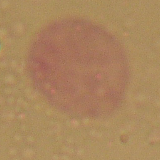
\includegraphics[width=0.95\linewidth]{Figures/Chapter2/1a.png}
	Оригінал
	\endminipage\hfill
	\minipage{0.2\textwidth}
	\centering	
	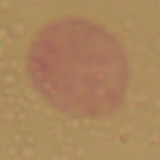
\includegraphics[width=0.95\linewidth]{Figures/Chapter2/1b.png}
	При \(k = 3\)
	\endminipage\hfill
	\minipage{0.2\textwidth}
	\centering	
	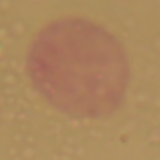
\includegraphics[width=0.95\linewidth]{Figures/Chapter2/1c.png}
	При \(k = 5\)
	\endminipage\hfill
	\minipage{0.2\textwidth}
	\centering	
	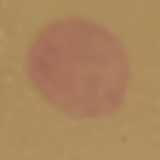
\includegraphics[width=0.95\linewidth]{Figures/Chapter2/1d.png}
	При \(k = 9\)
	\endminipage\hfill
	\minipage{0.2\textwidth}
	\centering	
	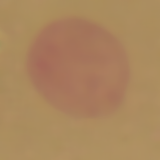
\includegraphics[width=0.95\linewidth]{Figures/Chapter2/1e.png}
	При \(k = 13\)
	\endminipage\hfill	
	
	\caption{Дія медіанного фільтру на зображення.}
	\label{fig:median_cells}
\end{figure}

На (Мал. \ref{fig:median_cells}) показано, як змінюється рівень шуму та чіткість зображення в залежності від розміру вікна фільтру \(k = 2r + 1\). Можна побачити, що при \(k = 3\), зображення мінімально позбавлене шуму, а текстура ядра майже повністю зберігається. При \(k = 13\) дуже гарно виділяються контури ядра клітини та зображення зовсім позбавлене шуму, але майже повністю втрачено текстуру ядра.

Отже, на різних етапах аналізу можна використовувати медіанні фільтри з різними розмірами вікна фільтру. Наприклад, при сегментації зображень (Мал. \ref{fig:raw_cells}) доречно використовувати вікна фільтру з великими розмірами, оскільки на цьому етапі нас більше цікавлять контури об'єктів, а при класифікації (здоровий, хворий раком або фіброаденоматозом) краще використовувати якомога менші вікна фільтру, оскільки нас цікавить текстура інтерфазного ядра клітини букального епітелію.


\subsection{Відділення фону. Бінаризація Оцу.}

\par
Наступний етап обробки зображення -- відділення фонових пікселів від пікселів об'єктів, наявних на зображенні (ядер клітин або сторонніх об'єктів). Для досягнення цієї мети підходить алгоритм бінаризації зображення Оцу \parencite{bib:otsu}. 

\par

Нехай пікселі зображення приймають значення у $L$ рівнях сірого кольору, тобто значення з множини $\left\{ 1, 2, \dots, L \right\}$, кількість пікселів зі значенням $i$ дорівнює $n_i$, а кількість пікселів у зображенні -- $N$. Треба розділити множину пікселів на два класи $C_0$ та $C_1$ (фонові пікселі та пікселі об'єктів, або навпаки) за допомогою деякого значення порогу $k$. До $C_0$ віднесемо усі пікселі зі значеннями з $\left\{ 1, 2, \dots, k \right\}$, а до $C_1$ -- усі пікселі зі значеннями з множини $\left\{ k+1, k+2, \dots, L \right\}$. Нехай $\omega_0$ та $\omega_1$ -- частота класів $C_0$ та $C_1$ відповідно.  

$$\omega_0 = \omega_0(k) = \sum_{i=0}^{k}{\frac{n_i}{N}}, \quad
\omega_1 = \omega_1(k) = \sum_{i=k+1}^{k}{\frac{n_i}{N}} = 1 - \omega_0$$

оді метод Оцу полягає у пошуку порогу $k$, який мінімізує дисперсію в середині класу, яка визначається як зважена сума дисперсій двох класів:

$$\sigma_{\omega}^{2}(k) = \sigma_{0}^2(k) \omega_0(k) + \sigma_{1}^2(k) \omega_1(k) \rightarrow \min$$

Де $\sigma_{0}^2(k)$ та $\sigma_{2}^2(k)$ -- дисперсія класів $C_0$ та $C_1$ для порогу $k$ відповідно. У своїй роботі Оцу також показав, що мінімізація дисперсії в середині класу рівносильна максимізації дисперсії між класами:

$$\sigma_{b}^2(k) = \omega_0(k)\omega_1(k) \left( \mu_0(k) - \mu_1(k) \right)^2 \rightarrow \max$$

Де $\mu_0(k)$ та $\mu_1(k)$ -- середнє арифметичне класів $C_0$ та $C_1$ при порозі $k$ відповідно, тобто:

$$\mu_T = {{\sum^{L}_{i=0} {i \cdot n_i}} \over {N}} $$
$$\mu_0(k) = {{\sum^{t-1}_{i=0} {i \cdot n_i}} \over {N \cdot \omega_0(k)}}, \quad \mu_1(t) = {{\mu_T - \mu_0(k) \cdot \omega_0(k)} \over {\omega_1(k)}}.$$

Значення $\omega_0(k+1)$, $\omega_1(k+1)$, $\mu_0(k+1)$ та $\mu_1(k+1)$ достатньо легко виражаються через значення $\omega_0(k)$, $\omega_1(k)$, $\mu_0(k)$ та $\mu_1(k)$, що дозволяє швидко обчислити оптимальний поріг $k$. Отже, алгоритм бінаризації Оцу виглядає наступним чином:

\begin{megaalgorithm}[H]
	\caption{Бінаризація зображення Оцу}
	\SetKwInOut{Input}{Вхід}\SetKwInOut{Output}{Вихід}
	
	\Input{Зображення $X$ розміром $m \times n$}
	\Output{Поріг $k$}
	\BlankLine 
	
	\textbf{обчислити} гістограму $n_i$ зображення та частоту $N(i) = \frac{n_i}{N}$ для кожного рівня інтенсивності зображення $X$\;
	\textbf{обчислити} початкові значення $\omega_0(0)$, $\omega_1(0)$, $\mu_0(0)$ та $\mu_1(0)$\;
	\textbf{поставити} $\sigma_{\max}^2 \leftarrow 0$\;
	\For{$k = 1 \textup{ to } L $}{
		\textbf{Оновити} значення $\omega_0(k)$, $\omega_1(k)$, $\mu_0(k)$ та $\mu_1(k)$\;
		\textbf{Обчислити} $\sigma_{b}^2(k) = \omega_0(k)\omega_1(k) \left( \mu_0(k) - \mu_1(k) \right)^2$\;		
		\If{$\sigma_{b}^2(k) > \sigma_{\max}^2$}{
			\textbf{поставити} $\sigma_{\max}^2 \leftarrow \sigma_{b}^2(k)$
		}
	}
	\textbf{поставити} $k \leftarrow \sigma_{\max}^2$\;
\end{megaalgorithm}

\begin{figure}[t!]
	\minipage{0.5\textwidth}
	\centering
	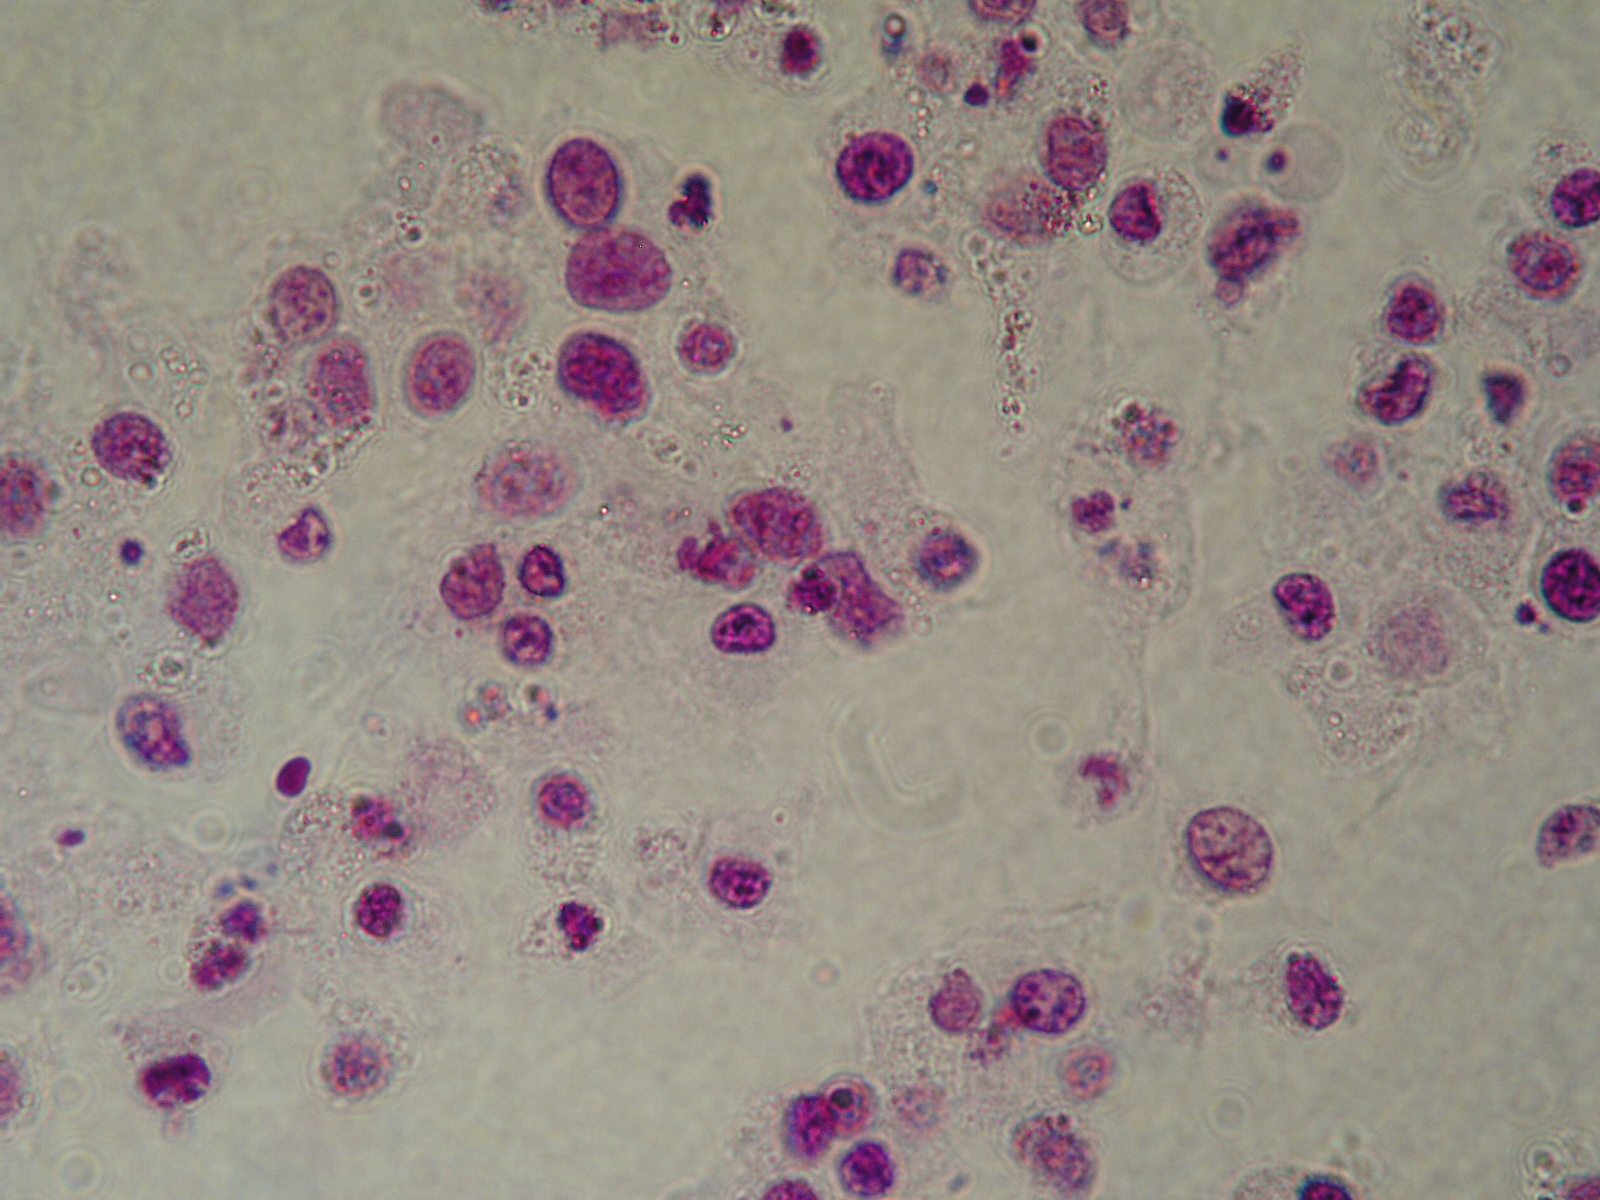
\includegraphics[width=0.97\linewidth]{Figures/Chapter2/2a.png}
	\endminipage\hfill
	\minipage{0.5\textwidth}
	\centering	
	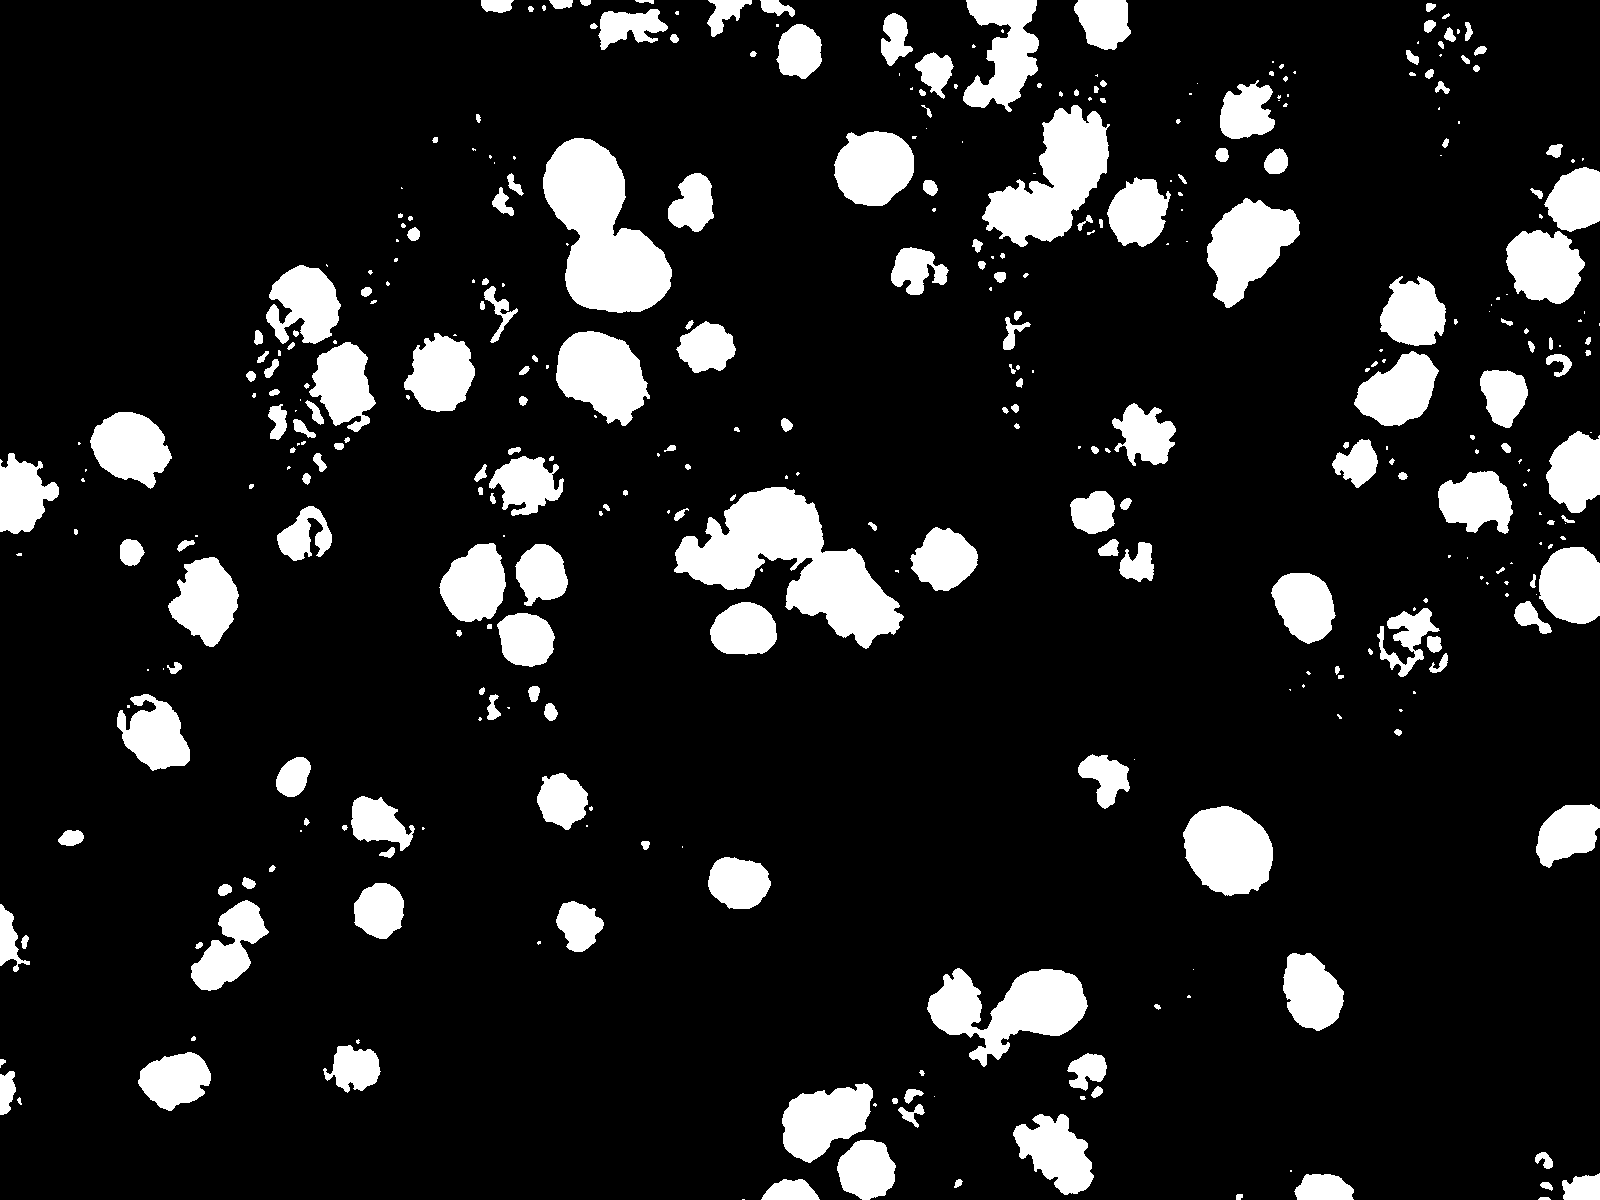
\includegraphics[width=0.97\linewidth]{Figures/Chapter2/2b.png}
	\endminipage\hfill	
	
	\caption{Результат бінаризації.}
	\label{fig:binarized_cells}
\end{figure}

\par
На зображенні (Мал. \ref{fig:binarized_cells}) результат бінаризації фільтрованого медіанним фільтром зобра- ження з розміром \(k = 5\). Негладкі контури інтерфазних ядер клітин після бінаризації, а також неточності у деяких регіонах зображення нас не турбують на даному етапі, оскільки це можна виправити морфологічними операціями, які будуть детально розгля- нуті далі.


\subsection{Бінарні морфологічні операції над зображеням.}

У бінарній морфології, зображення розглядається як підмножина Евклідового простору \(\mathbb{R}^d\) або цілочисельної сітки \(\mathbb{Z}^d\), де \(d\) -- розмірність простору. Операції морфології застосо- вуються до зображень разом з заданим структурним елементом, або ядром, яке визначає природу операції. Для обробки зображень найчастіше використовують наступний струк- турний елемент:
\begin{equation*}
B = \{ (-1, -1), (-1, 0), (-1, 1), (0, -1), (0, 0), (0, 1), (1, -1), (1, 0), (1, 1)\}\,.
\end{equation*}

Двома основними морфологічними операціями є Erosіon(звуження) і Dіlatіon(розширення). Операція звуження зображення задається наступним чином:
\begin{equation*}
A \ominus B = \left\{ z \in \mathbb{Z}^d | B_z \subseteq A \right\}\,,
\end{equation*}
де \(A\) -- зображення, \(B\) -- структурний елемент, \(B_z\) -- трансляція вектору \(z\), тобто
\begin{equation*}
B_z = \left\{ b + z | b \in B \right\}, \quad \forall z \in \mathbb{Z}^d
\end{equation*}

Ідея цієї операції полягає в наступному. Ядро (структурний елемент) ковзає по зобра- женню. Піксель в бінаризованому зображенні (1 або 0) буде вважатися 1, тільки якщо всі пікселі під ядром рівні 1, в іншому випадку він буде зруйнований (стане рівним нулю). Таким чином, в результаті операції всі пікселі, що знаходяться на краю, будуть відкинуті в залежності від розміру ядра. Таким чином, товщина або розмір об'єкта переднього плану зменшується. Цей метод може використовуватися для видалення невеликих шумів, роз’єднання двох пов'язаних об'єктів та іншого.

Операція розширення зображення задається наступним чином:
\begin{equation*}
A  \oplus B = \bigcup_{b\in B} A_b\,.
\end{equation*}

Ця операція протилежна ерозії. Тут піксель бінаризованого зображення  дорівнює \enquote{1}, якщо принаймні один піксель під ядром дорівнює \enquote{1}. Таким чином, збільшується біла область зображення або збільшується розмір об'єкта переднього плану. Зазвичай у ви- падках, коли потрібно видалити шум навколо об’єкта, спочатку використовують опера- цію звуження, а потім операцію розширення. Розширення необхідне, оскільки ерозія, крім видалення білого шуму, скорочує наш об'єкт. 

\begin{figure}[t!]
	\minipage{0.333\textwidth}
	\centering
	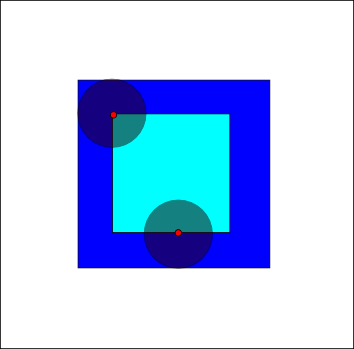
\includegraphics[width=0.80\linewidth]{Figures/Chapter2/Erosion.png}
	Звуження \(\ominus\)
	\endminipage\hfill
	\minipage{0.333\textwidth}
	\centering	
	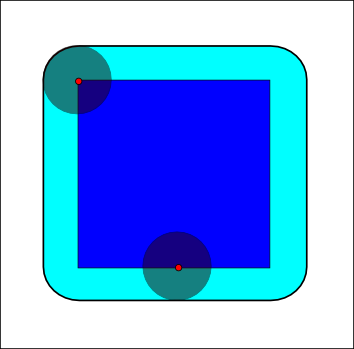
\includegraphics[width=0.80\linewidth]{Figures/Chapter2/Dilation.png}
	Розширення \(\oplus\)
	\endminipage\hfill
	\minipage{0.333\textwidth}
	\centering	
	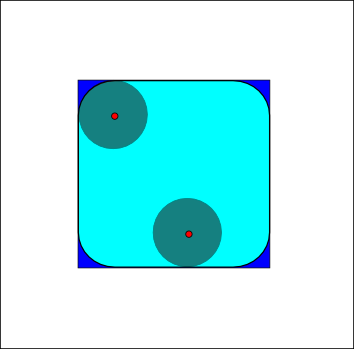
\includegraphics[width=0.80\linewidth]{Figures/Chapter2/Opening.png}
	Відкриття \(\circ\)
	\endminipage\hfill
	
	\caption{Морфологічні операції з круглим структурним елементом над синім квадратом.}
	\label{fig:morphology_explained}
\end{figure}

На основі основних операцій звуження (\(\ominus\)) та розширення (\(\oplus\)) задаються інші операції. Операція морфологічного відкриття (openіng) задається наступним чином:
\begin{equation*}
A \circ B  = (A \ominus B) \oplus B\,.
\end{equation*}

або
\begin{equation*}
A \circ Bс = \mathop\bigcup\limits_{B_{{\textbf{z}}}\subseteq A} {B_{{\textbf{z}}}}.
\end{equation*}

У \citep{book:serra} більш детально розглянуто теоретичні та практичні аспекти операції математичної морфології.

Позначимо зображення, отримане у результаті розширення бінарного зображення за 2 ітерації у (\ref{fig:morph_cells}) як \(zoneOfinterest\). Очевидно, що всі пікселі, які дорівнюють \(0\) у \(sureBG\) є пікселями фону. Отже, ядра треба шукати тільки серед тих точок \(zoneOfinterest\), які дорівнюють \(1\) (позначено білим кольором). Позначимо також відкриття у (Мал. \ref{fig:morph_cells}) як \(threshOpenіng\).

\begin{figure}[b!]
	\minipage{0.5\textwidth}
	\centering	
	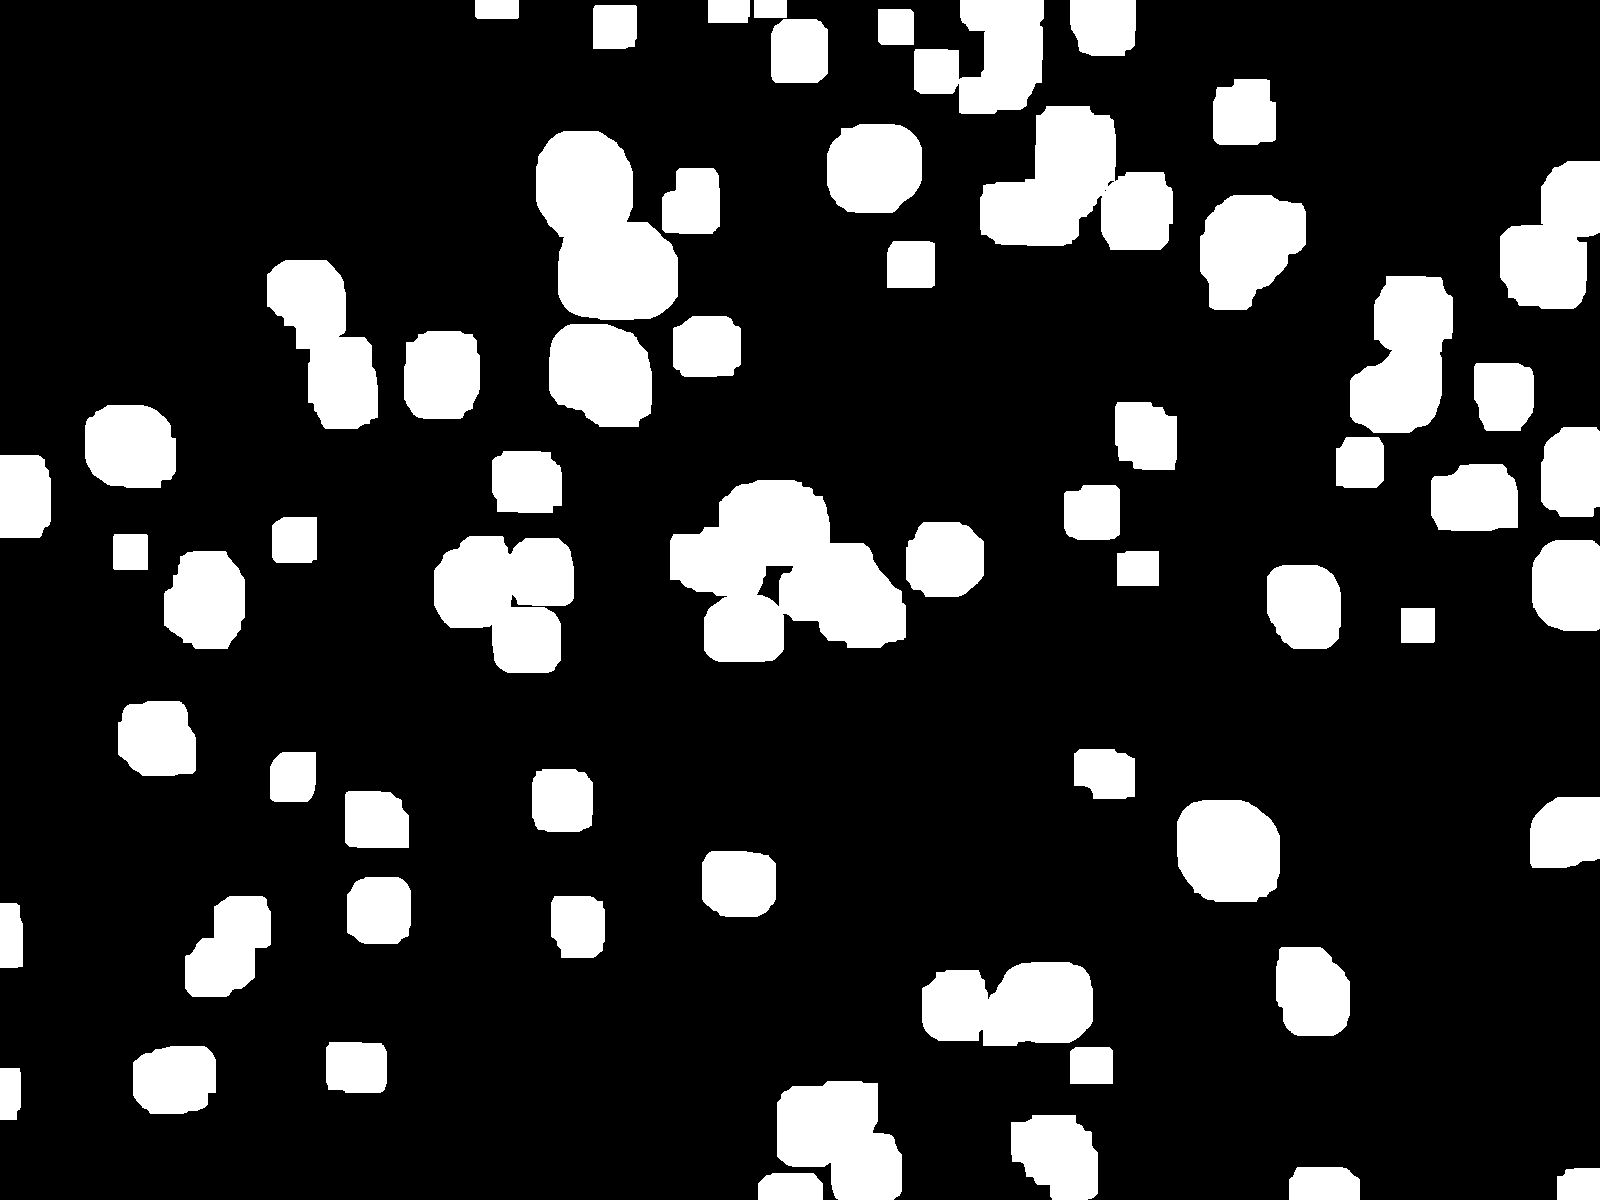
\includegraphics[width=0.95\linewidth]{Figures/Chapter2/3a.png}
	Розширене зображення за 2 ітерації
	\endminipage\hfill
	\minipage{0.5\textwidth}
	\centering	
	
\includegraphics[width=0.95\linewidth]{Figures/Chapter2/3b.png}
	Відкриття зображення за 2 ітерації
	\endminipage\hfill
	
	\caption{Морфологічні операції над бінарним зображенням (Мал. \ref{fig:binarized_cells}).}
	\label{fig:morph_cells}
\end{figure}


\subsection{Трансформація дистанції}

\begin{figure}[t!]
	\minipage{0.5\textwidth}
	\centering	
	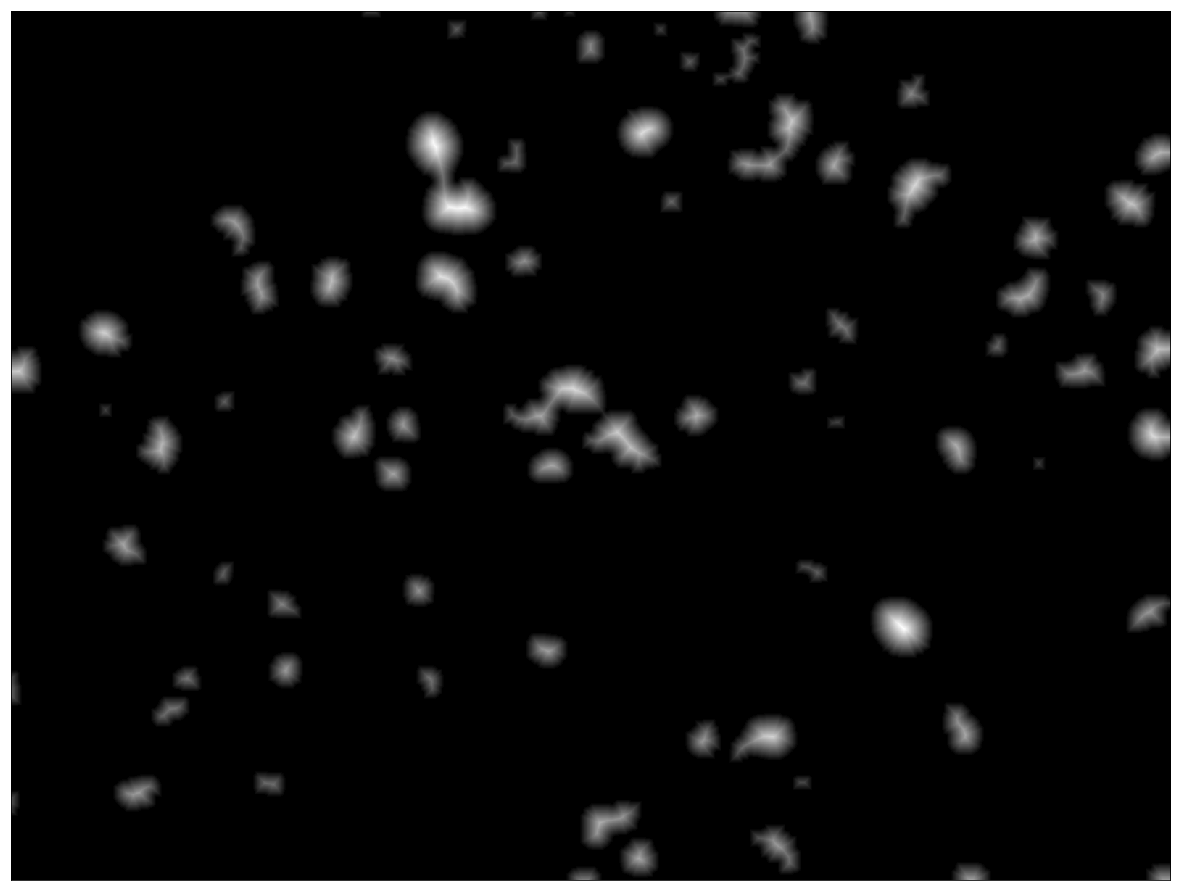
\includegraphics[width=0.95\linewidth]{Figures/Chapter2/4a.png}
	Трансформація дистанції
	\endminipage\hfill
	\minipage{0.5\textwidth}
	\centering	
	
\includegraphics[width=0.95\linewidth]{Figures/Chapter2/4b.png}
	\(sureFG\)
	\endminipage\hfill
	
	\caption{Трансформація дистанції.}
	\label{fig:dist_transform}
\end{figure}

Трансформація дистанції (Dіstance Transformatіon) є також операцією математичної мор- фології. Кожному пікселю переднього плану (що належить \(E\)) бінарного зображення \(E \subseteq \mathbb{Z}^d\) ставиться у відповідність відстань цієї точки до найближчого пікселя заднього плану (що не належить \(E\)). Для бінарних зображень найчастіше використовують Евклідову відстань, тобто для зображення \(E \subseteq F = \{1, 2, \dots, heіght\} \times \{1, 2, \dots, wіdth\}\), кожній точці \(z = (z_x, z_y) \in E\) ставимо у відповідність:
\begin{equation*}
DT(z) = \inf_{(x, y) \in F}{(|x - z_x| + |y - z_y|)}
\end{equation*}

Результат цієї операції для \(E = threshOpenіng\) можна інтерпретувати як показник вірогідності, що піксель \(z = (z_x, z_y)\) належить інтерфазному ядру клітини букального епітелію. Отже, можна задати емпіричне правило, за яким будемо приймати певні пікселі як \enquote{точно належать ядру клітини}:
\begin{equation}\label{eq:sure_fg}
DT(z) \geq \alpha \cdot \sup_{s \in E}{DT(s)} \Rightarrow \text{\enquote{z точно належать ядру клітини}}.
\end{equation}

Позначимо множину, що задовольняє цю нерівність, як \(sureFG\). Множник \(\alpha = 0.475\) був обраний експериментальним чином, на досліджуваних даних. Тут також використо- вується припущення, що усі ядра клітин мають приблизно однаковий розмір, а отже, центри цих клітин будуть знаходитись на приблизно однакому відстані від точок заднього плану. Для інших задач, дані яких зібрані за інших умов, слід обрати інший множник.

У (\ref{fig:dist_transform}) показано результат трансформації відстані та обчислення \(sureFG\) над бінарним зображенням \(threshOpenіng\), зображеним на (\ref{fig:morph_cells}). На \(sureFG\) ядра не дотикаються, завдяки обраному параметру \(\alpha\), тобто наш метод сегментації коректно обробляє ситуації, коли клітини торкаються чи частково перекриваються.

Використовуючи алгоритм що запропонований у \citep{bib:cooldisttrans} який використовує так звану рекур- сивну морфологію, можна обчислити трансформацію дистанції за два обходу. Для пов- ного виявлення окремих клітин, використаємо алгоритм водоподілу.

\subsection{Алгоритм водоподілу}

Трансформація водоподілу (Watershed) розглядає одноканальне зображення як топогра- фічну карту, де значення пікселя відображає висоту цієї точки. 

Починаючи з точок локальних мінімумів (або з заданих точок), кожна “яма” запов- нюється рідиною різних кольорів. З підвищенням рівня рідини, настає момент, коли дві рідини різного кольору починають змішуватися. Щоб уникнути цього, будуються границі між регіонами цих рідин. Границі будуються, доки рівень рідини не стане вищим за найвищу точку карти. Побудовані границі є результатами сегментації.

Використаємо цю ідею для сегментації ядер клітин. Кожну зв'язну компоненту \(sureFG\) пофарбуємо в певний \enquote{колір}. Назвемо таку сегментацію \enquote{набором маркерів}. Позначимо
\begin{equation*}
sureBG = E \setminus zoneOfInterest
\end{equation*}

Зв'язну множину пікселів заднього плану \(sureBG\) також пофарбуємо в якийсь колір. Непофарбованою залишається така множина:
\begin{equation*}
unknownRegion = zoneOfInterest \setminus sureFG
\end{equation*}

Тоді алгоритм водоподілу з заданими маркерами наступний \citep{bib:watershed}:

\begin{megaalgorithm}[H]
	\caption{Алгоритм водоподілу Майера з заданими маркерами}
	\SetKwInOut{Input}{Вхід}\SetKwInOut{Output}{Вихід}
	
	\Input{Зображення $X$ розміром $m \times n$, набір маркерів}
	\Output{Сегментація}
	\BlankLine 
	
	0. Будемо вважати, що \enquote{затоплення} починається саме с пікселів маркерів.\;
	1. Сусідні пікселі кожного маркеру додаємо в чергу з пріоритетом, де рівень пріоритету залежить від величини градієнту пікселя.\;
	2. Розглядається піксель з найменшим рівнем пріоритету. Якщо сусідні пікселі вже пофарбовані та мають однаковий колір, то фарбуємо цей піксель у колір сусідів. Усі сусіди, які ще не пофарбовані та ще не належать до черги з пріоритетом, додаються у чергу.\;
	3. Повторюємо крок 2, поки черга не стане пустою.\;
	4. Незафарбовані пікселі є границями водоподілу.\;
\end{megaalgorithm}

\begin{figure}[t!]
	\minipage{0.5\textwidth}
	\centering	
	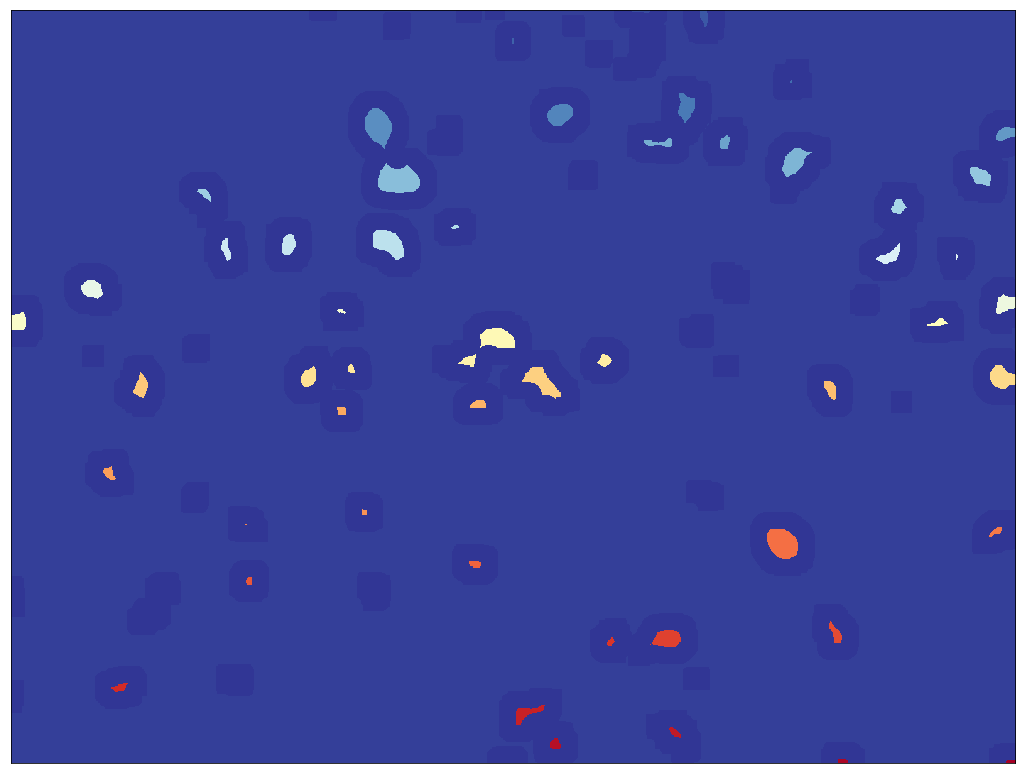
\includegraphics[width=0.95\linewidth]{Figures/Chapter2/5a.png}
	Маркери
	\endminipage\hfill
	\minipage{0.5\textwidth}
	\centering	
	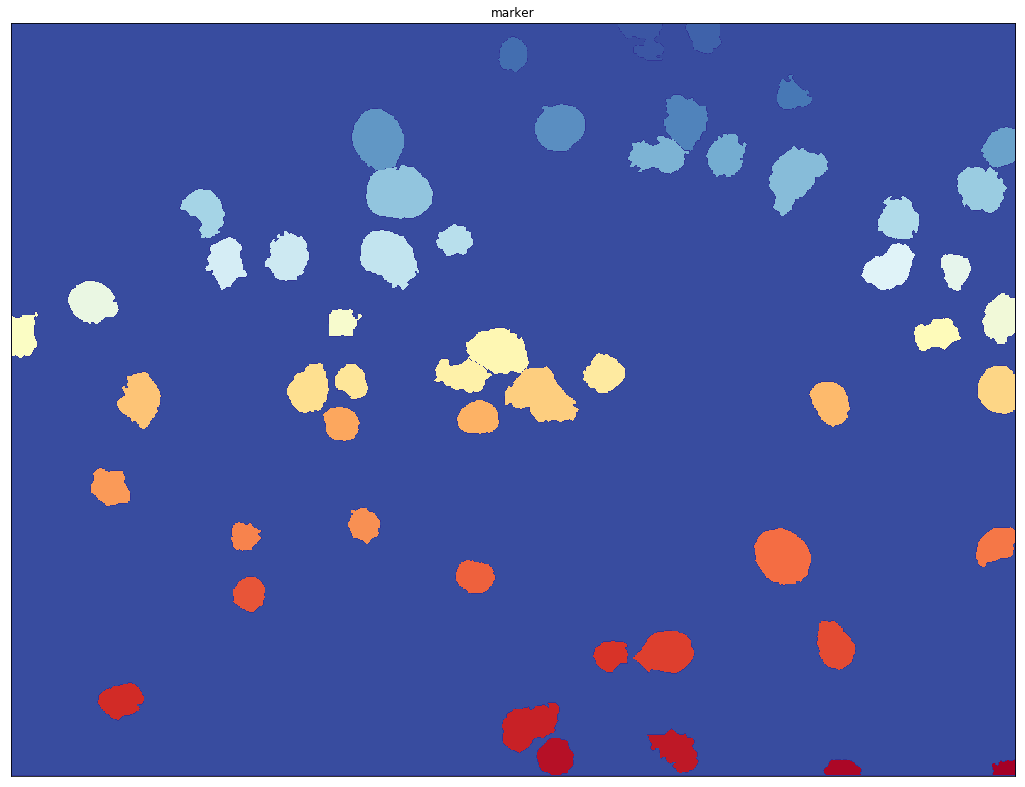
\includegraphics[width=0.95\linewidth]{Figures/Chapter2/5b.png}
	Кінцевий результат сегментації
	\endminipage\hfill
	
	\caption{Результат роботи алгоритму водоподілу (watershed).}
	\label{fig:watershed}
\end{figure}

\subsection{Кінцевий алгоритм сегментації}

Отже, кінцевий алгоритм сегментації інтерфазних ядер букального епітелію виглядає наступним чином:

\begin{megaalgorithm}[H]
	\caption{Сегментація ядер}
	\SetKwInOut{Input}{Вхід}\SetKwInOut{Output}{Вихід}
	
	\Input{Зображення $X$ розміром $m$}
	\Output{Зображення $Y$ такого ж розміру, де різні ядра зображені різними кольорами}
	\BlankLine 
	
	\(gray \leftarrow \text{сіре зображення X (grayscale)} \)\;
	\(blured \leftarrow \text{медіанна фільтрація }\, gray\, \text{ з вікном радіусом }\, r = 2\)\;
	\(thresh \leftarrow \text{бінаризація Оцу для }\, blured\)\;
	\(threshOpenіng \leftarrow\) морфологічне відкриття \(thresh\) з ядром \(9 \times 9\) за 2 ітерації\;
	\(zoneOfіnterest \leftarrow\) морфологічне розширення \(openіng\) з ядром \(9 \times 9\) за 2 ітерації\;
	\(dіstTransform \leftarrow\) трансформація відстані для \(threshOpenіng\)\;
	\(sureFG \leftarrow z\), які задовольняють формулу (\ref{eq:sure_fg})\;
	\(unknownRegіon \leftarrow zoneOfіnterest \setminus sureFG\)\;
	\(markers \leftarrow\) зв'язні компоненти \(sureFG \cup sureBG\)\;
	Виконати алгоритм водоподілу.
	
\end{megaalgorithm}

\begin{figure}[t!]
	\minipage{0.25\textwidth}
	\centering	
	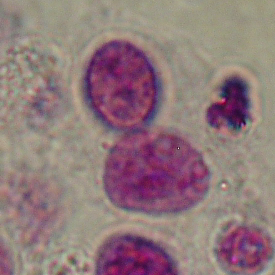
\includegraphics[width=0.97\linewidth]{Figures/Chapter2/6a1.png}
	
\includegraphics[width=0.97\linewidth]{Figures/Chapter2/6b1.png}
	
\includegraphics[width=0.97\linewidth]{Figures/Chapter2/6c1.png}
	\endminipage\hfill
	\minipage{0.25\textwidth}
	\centering	
	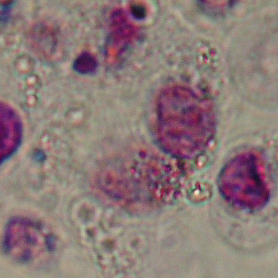
\includegraphics[width=0.97\linewidth]{Figures/Chapter2/6a2.png}	
	
\includegraphics[width=0.97\linewidth]{Figures/Chapter2/6b2.png}	
	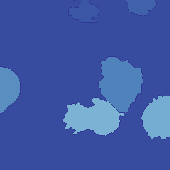
\includegraphics[width=0.97\linewidth]{Figures/Chapter2/6c2.png}
	\endminipage\hfill
	\minipage{0.25\textwidth}
	\centering	
	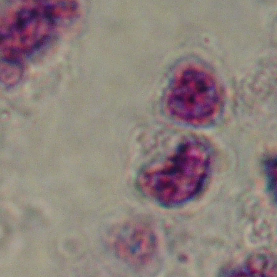
\includegraphics[width=0.97\linewidth]{Figures/Chapter2/6a3.png}	
	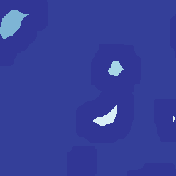
\includegraphics[width=0.97\linewidth]{Figures/Chapter2/6b3.png}	
	
\includegraphics[width=0.97\linewidth]{Figures/Chapter2/6c3.png}
	\endminipage\hfill
	\minipage{0.25\textwidth}
	\centering	
	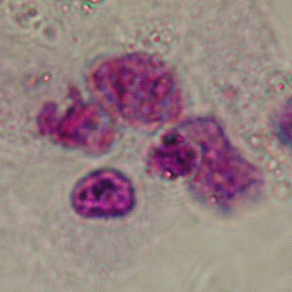
\includegraphics[width=0.97\linewidth]{Figures/Chapter2/6a4.png}	
	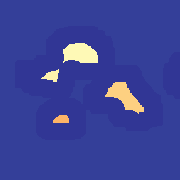
\includegraphics[width=0.97\linewidth]{Figures/Chapter2/6b4.png}	
	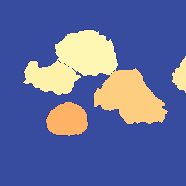
\includegraphics[width=0.97\linewidth]{Figures/Chapter2/6c4.png}
	\endminipage\hfill
	
	\caption{Випадки, коли ядра торкаються чи частково перекриваються.}
	\label{fig:amazing_segmentation}
\end{figure}

\bigskip
На (Мал. \ref{fig:amazing_segmentation}) бачимо, що наш алгоритм коректно сегментує також ті випадки, коли ядра клітин торкаються одне одного.

%----------------------------------------------------------------------------------------
%	SECTION 2

%----------------------------------------------------------------------------------------

\section{Нормалізація зображень}

Для нейронної мережі важливо переконатися, що вхідні дані нормалізовані. Для випадку зображень інтерфазних ядер букального епітелію, зображення можуть бути отримані у трохи різних умовах. Це може вплинути на швидкість тренування нейронної мережі, а також на точність розпізнавання.

Задньому плану зображення присвоюємо значення \(0\), щоб воно не активувало нейрони у мережі. Виконуємо нормалізацію гістограми для зображення одного ядра клітини так, щоб пікселі ядра приймали значення від \(0\) до \(255\). Це також може надати прискорення тренуванню нейронної мережі, оскільки більший діапазон значень означає більшу різ- ницю градієнтів у різних точках зображення.

Використовуючи попередні результати, видалимо задній план із зображення. Ядро клі- тини нормалізуємо за допомогою еквалізації гістограми, результат показано на  (Мал. \ref{fig:normalized_cells}).


\begin{figure}[t!]
	\minipage{0.2\textwidth}
	\centering
	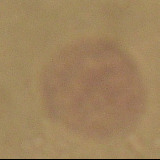
\includegraphics[width=0.95\linewidth]{Figures/Chapter2/7a1.png}	
	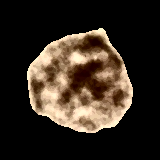
\includegraphics[width=0.95\linewidth]{Figures/Chapter2/7a2.png}	
	\endminipage\hfill
	\minipage{0.2\textwidth}
	\centering	
	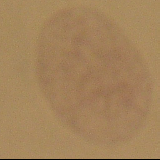
\includegraphics[width=0.95\linewidth]{Figures/Chapter2/7b1.png}
	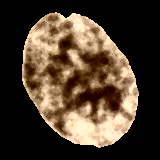
\includegraphics[width=0.95\linewidth]{Figures/Chapter2/7b2.png}
	\endminipage\hfill
	\minipage{0.2\textwidth}
	\centering	
	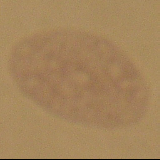
\includegraphics[width=0.95\linewidth]{Figures/Chapter2/7c1.png}
	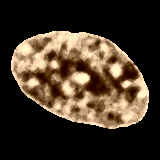
\includegraphics[width=0.95\linewidth]{Figures/Chapter2/7c2.png}
	\endminipage\hfill
	\minipage{0.2\textwidth}
	\centering	
	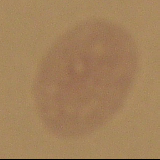
\includegraphics[width=0.95\linewidth]{Figures/Chapter2/7d1.png}
	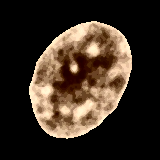
\includegraphics[width=0.95\linewidth]{Figures/Chapter2/7d2.png}
	\endminipage\hfill
	\minipage{0.2\textwidth}
	\centering	
	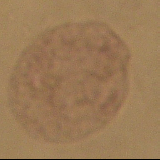
\includegraphics[width=0.95\linewidth]{Figures/Chapter2/7e1.png}
	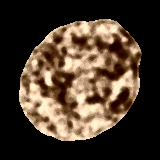
\includegraphics[width=0.95\linewidth]{Figures/Chapter2/7e2.png}
	\endminipage\hfill	
	
	\caption{Нормалізація зображень.}
	\label{fig:normalized_cells}
\end{figure}

%----------------------------------------------------------------------------------------
%	SECTION 4
%----------------------------------------------------------------------------------------

\section{Фільтр на основі еліпсоїдів Петуніна}

Згідно з роботою \parencite{bib:petuninfilter}, фільтр зображень на основі використання еліпсоїдів Петуніна має багато переваг над медіанним фільтром. У випадку фільтрації зображень інтерфазних ядер клітин, цей метод краще зберігає форму текстури. Отже, його можна використо- вувати для попередньої обробки даних для фрактального аналізу.

\subsection{Еліпсоїди Петуніна}

Нехай маємо множину точок \(M = \left\{x_1, x_2, \dots, x_n\right\}\), де \(x_i \in \mathbb{R}^m\) -- множина точок у \(m\)-вимірному просторі. Знайдемо точки \(x_l, x_k\) такі, щоб
\begin{equation*}
\sup_{x_i, x_j \in M}{\|x_i - x_j\|} = \|x_l - x_k\|
\end{equation*}
тобто відрізок \(L = x_l x_k\) -- діаметр множини точок \(M\). Повернемо і перенесемо систему координат так, щоб діаметр \(L\) належав \(O_{x'_1}\), де \(x'_1, x'_2, \dots, x'_n\) -- координати множини \(M\) у новій системі координат. 

Побудуємо найменший прямокутний паралелепіпед у \(\mathbb{R}^m\), який містив би елементи мно- жини \(M' = \left\{x'_1, x'_2, \dots, x'_n\right\}\). Стискаючи цей найменший прямокутний паралелепіпед, відобразимо його точки у гіперкуб. Знайдемо центр \(x_0\) гіперкуба та обчислимо відстані \(r_1, r_2, \dots, r_n\) від нього до кожної точки. 

Знайдемо найбільше \(R = \max{(r_1, r_2, \dots, r_n)}\) та побудуємо гіперкулю навколо центру \(x_0\) з радіусом \(R\). Зробимо обернене перетворення розтягу, повороту та переносу, отримаємо еліпсоїд Петуніна у \(m\)-вимірному просторі для множини \(M\). Система еліпсоїдів, отрима- них з кіл радіусами \(r_i\), де \(i \in 1, \dots n\) називається концентрованою системою еліпсоїдів Петуніна для множини \(M\).

Для системи концентрованих еліпсоїдів також справжується властивості, що є наслід- ками роботи Хілла \citep{bib:hill} та детально описані та доведені у \citep{bib:lyashko}.

\subsection{Фільтр зображень на основі еліпсоїдів Петуніна}

Нехай маємо на вході зображення, кожен піксель якого має \(d\) каналів. Зображення розглядається як відображення \(M: \mathbb{Z^2} \rightarrow \mathbb{R}^d\), тобто кожній координаті присвоюється \(d\)-канальне значення. Для кожного пікселя зображення, розглядаємо ще декілька пікселів, координати яких знаходяться в радіусі \(r\) від цього пікселя. Побудуємо для множини значень цих пікселів концентровану систему еліпсоїдів Петуніна, та у вихідному зобра- женні присвоїмо пікселю з тими ж координатами значення, яке відповідає внутрішньому (або центральному) еліпсоїду.

Детальний алгоритм виглядає наступним чином:

\begin{megaalgorithm}[H] \label{alg:petuninfilter0}
	\caption{Фільтр Петуніна}
	\SetKwInOut{Input}{Вхід}\SetKwInOut{Output}{Вихід}
	
	\Input{Зображення $X$ розміром $w \times h$, радіус ядра (вікна фільтру) \(r\)}
	\Output{Зображення $Y$ такого ж розміру}
	\BlankLine 
	
		
	\For{\(i = 1 \textup{ to } w \)}{
		\For{\(j = 1 \textup{ to } h \)}{
			\(D \leftarrow \text{нескінченний відрізок}\)\;
			\For {\(k = -r \textup{ to } r\)}{
			\For {\(l = -r \textup{ to } r\)}{
			\For {\(o = -r \textup{ to } r\)}{
			\For {\(p = -r \textup{ to } r\)}{
				Якщо \(\|D\| < \|X_{i+k, j+l} - X_{i+o, j+p}\|\) то \(D \leftarrow X_{i+k, j+l} X_{i+o, j+p}\) 
			}}}}
			Побудувати систему концентрованих еліпсоїдів Петуніна, маючи діаметр \(D\)\;
			$Y_{i,j} \leftarrow \textup{значення, що відповідає внутрішньому (або центральному) еліпсоїду}$\;
		}		
	}
\end{megaalgorithm}


\subsection{Швидкий алгоритм на основі динамічного програмування}

Незважаючи на переваги фільтру на основі еліпсоїдів Петуніна над медіанним фільтром (Алгоритм \ref{alg:petuninfilter0}) має серйозний недолік. Так, для зображення розміром \(w \times h\) та фільтру радіусом \(r\), асимптотична оцінка швидкості цього алгоритму становить:
\begin{equation*}
O\left( w \cdot h \cdot r^4 \right).
\end{equation*}

Для порівняння, асимптотична оцінка швидкості швидкого алгоритму медіанної фільтра- ції (Алгоритм \ref{alg:medianfilter}) або фільтра Гауса становить
\begin{equation*}
O\left(
\min\{w, h\} \cdot r^2 + w \cdot h \cdot r
\right).
\end{equation*}

Отже, при великих розмірах ядра (наприклад, \(r > 10\)) та великому об'ємі зображень, фільтр зображень на основі еліпсоїдів Петуніна значно повільніше працює, ніж інші алгоритми фільтрації. Основна причина -- повільний пошук діаметру. 

Існує багато швидких алгоритмів пошуку діаметру множини точок у \(d\)-вимірному прос- торі. Так, наприклад, Har-Peled запропонував евристичний алгоритм знаходження діа- метру \citep{bib:harpeled}. У \citep{bib:diamset} запропоновано детермінований алгоритм, що дозволяє знайти діаметр за час \(O\left( n \log n \right)\), де \(n\) -- кількість точок множини. Недоліком цих алгоритмів при викорис- танні для фільтру на основі еліпсоїдів Петуніна є те, що незважаючи на меншу асимпто- тику, ці алгоритми при невеликої кількості точок працюють не швидше, ніж простий алгоритм (повний перебір) пошуку діаметру. Оскільки розміри фільтрів більших ніж 21 майже не мають практичного використання, ми не можемо використовувати ці алгоритми для прискорення процесу пошуку діаметру.

Можна помітити, що при \enquote{пересування} вікна фільтру, ми повторно виконуємо деякі обчислення. Якщо зможемо оптимальніше виконувати обчислення (без повторень), то зможемо швидше фільтрувати зображення. Автором цієї роботи пропонується алгоритм на основі динамічного програмування, що значно прискорює процес пошуку діаметру.

Опишемо структуру даних \enquote{двовимірна черга що зберігає діаметр}. Ця структура пред- ставляє собою двійка \(\left(H, p\right)\), де p -- координата центру вікна фільтру відносно зображення \(X\), а H -- таблиця розміром \((2r + 1) \times (2r + 1)\), кожен елемент якого зберігає діаметр множини точок, що відповідає пікселям, що потра- пляють у фільтр нижче чи правіше, тобто:
\begin{equation}
\label{eq:queueinit}
H_{i, j} = \left\| D(\{ X_{y, x} \big| x \in [(p_x + i), (p_x + r)]_{\mathbb{Z}}, y \in [(p_y + j), (p_y + r)]_\mathbb{Z} \}) \right\|,\,\, i, j \in -r \dots r
\end{equation}

\par
де \(D\) -- діаметр множини, \(X_{y, x}\) -- \(d\)-вимірне значення пікселю з координатами \((y, x)\). Очевидно, що в \(H_{-r, -r}\) зберігається діаметр множини точок значень пікселів, що потра- пляють у вікно фільтру. 

\par
Опишемо алгоритм оновлення таблиці \(H\) при пересуванні фільтру праворуч. Алгоритм при пересуванні фільтру вниз задається аналогічним чином.

\bigskip

\begin{megaalgorithm}[H] \label{alg:2dqueuetranslation}
	\caption{Оновлення таблиці \(H\) при пересуванні вікна фільтру праворуч}	
	\SetKwInOut{Input}{Вхід}\SetKwInOut{Output}{Вихід}
	
	\Input{Зображення $X$, радіус ядра (вікна фільтру) \(r\), двовимірна черга що зберігає діаметр \((H, p)\) що відповідає вікну}
	\Output{двовимірна черга що зберігає діаметр \((H', p')\) що відповідає вікну після зміщення праворуч на 1 піксель}
	\BlankLine 
	
	\(H'_{r, r} \leftarrow 0\)\;
	\For{\(i = r - 1 \textup{ downto } -r\)}{
		\(H'_{r, j} \leftarrow \max\left\{ \max\left\{ \|X_{p_y+i, p_x+r} - X_{p_y+k, p_x+r}\| \quad \forall k \in i \dots r \right\}, \quad H'_{i+1, r} \right\}\)
	}
	\For{\(j = r - 1 \textup{ downto } -r\)}{
		\For{\(i = r \textup{ downto } -r\)}{
			\(H'_{i,j} \leftarrow \max\left\{ \max\left\{ \|X_{p_y+i,p_x+j} - X_{p_y+k, p_x+r}\| \quad \forall k \in i \dots r \right\}, \quad H'_{i+1, j}, \quad H'_{i, j+1} \right\}\)
		}
	}
\end{megaalgorithm}

Також опишемо алгоритм для обчислення \((H, p)\), знаючи \((H^{left}, p^{left})\) та \((H^{top}, p^{top})\), де \(p^{left} = (p_y, p_x-1)\), \(p^{top} = (p_y-1, p_x)\), тобто знаючи черги, що відповідають вікнам на піксель вище чи лівіше.

\begin{megaalgorithm}[H] \label{alg:2dqueueinstantiation}
	\caption{Обчислення таблиці \(H\) знаючи відповідні таблиці ліворуч та вище}	
	\SetKwInOut{Input}{Вхід}\SetKwInOut{Output}{Вихід}
	
	\Input{Зображення \(X\), радіус ядра (вікна фільтру) \(r\), двовимірні черги що зберігає діаметр \((H^{left}, p^{left})\) та \((H^{top}, p^{top})\) що відповідає вікну лівіше та вище відповідно}
	\Output{двовимірна черга що зберігає діаметр \((H, p)\)}
	\BlankLine 
	
	\(H_{r, r} \leftarrow 0\)\;
	\For{\(i = r \textup{ downto } -r\)}{
	\For{\(j = r \textup{ downto } -r\)}{
		\(H_{i,j} = \max\left\{
		H^{left}_{i, j+1}, \quad
		H^{top}_{i+1, j}, \quad
		H_{i, j+1}, \quad
		H_{i+1, j}, \quad
		\|X_{p_y+r, p_x+r} - X_{p_y+i, p_x+j}\|,
		\right\}\)
	}
	}
\end{megaalgorithm}

\par
Слід зазначити, що в (Алгоритм \ref{alg:2dqueuetranslation}) та (Алгоритм \ref{alg:2dqueueinstantiation}), після кожного кроку присвоєння значення діаметру, слід також у таблиці \(D_{i, j}\) зберігати точки кінців діаметру. Опишемо кінцевий алгоритм швидкої фільтрації зображення на основі системи концентрованих еліпсоїдів Петуніна:

\begin{megaalgorithm}[H] \label{alg:petuninfilter1}
	\caption{Швидкий алгоритм фільтрації Петуніна}
	\SetKwInOut{Input}{Вхід}\SetKwInOut{Output}{Вихід}
	
	\Input{Зображення \(X\) розміром \(w \times h\), радіус ядра (вікна фільтру) \(r\)}
	\Output{Зображення \(Y\) такого ж розміру}
	\BlankLine 
	
	Обчислити \((H_0, p_0 = (1, 1))\) згідно за формулою (\ref{eq:queueinit}), а також відповідний відрізок \(L_0\)\;
	\For{\(i = 1 \textup{ to } h \)}{
		За (Алгоритм \ref{alg:2dqueuetranslation}) обчислити \((H^{i, 1}, p^{i, 1} = (i, 1))\) та відповідний відрізок \(L^{i, 1}\)\;
		Побудувати систему концентрованих еліпсоїдів Петуніна, маючи діаметр \(L^{i,1}\)\;
		$Y_{i,1} \leftarrow \textup{значення, що відповідає внутрішньому (або центральному) еліпсоїду}$\;
	}
	\For{\(j = 1 \textup{ to } w \)}{
		За (Алгоритм \ref{alg:2dqueuetranslation}) обчислити \((H^{1, j}, p^{1, j} = (1, j))\) та відповідний відрізок \(L^{1, j}\)\;
		Побудувати систему концентрованих еліпсоїдів Петуніна, маючи діаметр \(L^{1,j}\)\;
		$Y_{1,j} \leftarrow \textup{значення, що відповідає внутрішньому (або центральному) еліпсоїду}$\;
	}

	\For{\(i = 1 \textup{ to } h \)}{
		\For{\(j = 1 \textup{ to } w \)}{
			За (Алгоритм \ref{alg:2dqueueinstantiation}) обчислити \((H^{i, j}, p^{i, j})\) та відповідний відрізок \(L^{i,j}\)\;
			Побудувати систему концентрованих еліпсоїдів Петуніна, маючи діаметр \(L^{i,j}\)\;
			$Y_{i,j} \leftarrow \textup{значення, що відповідає внутрішньому (або центральному) еліпсоїду}$\;
		}		
	}
\end{megaalgorithm}

\par
Очевидно, що (Алгоритм \ref{alg:2dqueuetranslation}) має асимптотичну оцінку \(O\left( r^3 \right)\), а (Алгоритм \ref{alg:2dqueueinstantiation}) має оцінку \(O\left(r^2\right)\). Тоді асимптотична оцінка для (Алгоритм \ref{alg:petuninfilter1}) дорівнює:
\begin{equation*}
O\left(
r^4 + r^3 \left(w + h\right) + w \cdot h \cdot r^2
\right)
\end{equation*}

Оскільки значення \(r\) значно менша ніж розмір зображення \(w \times h\), то (Алгоритм \ref{alg:petuninfilter1}) можна оцінити як
\begin{equation*}
O\left(w \cdot h \cdot r^2\right)
\end{equation*}

Що дорівнює швидкості звичайного алгоритму медіанної фільтрації.
%\include{Chapters/Chapter25}
% Chapter Template

\chapter{Фрактальний аналіз} % Main chapter title

\label{Chapter3} % Change X to a consecutive number; for referencing this chapter elsewhere, use \ref{ChapterX}

%----------------------------------------------------------------------------------------
%	SECTION 1
%----------------------------------------------------------------------------------------

Наступним етапом цієї роботи є обчислення фрактальної розмірності для попередньо оброблених зображень. Таким чином, для кожного \textit{пацієнта} буде побудовано набір фрак- тальних характеристик.

\section{Фрактальна характеристика}
\subsection{Теоретичні відомості}

Для визначення поняття фракталу треба спочатку навести визначення розмірності Хаус- дорфа. Нехай $\Omega$ -- обмежена множина у метричному просторі $X$.

\begin{defn}
	Нехай $\epsilon > 0$. Не більш ніж зліченне сімейство $\left\{ \omega_i \right\}_{i \in I}$ підмножин простору $X$ будемо називати \textbf{$\epsilon \textit{-покриттям}$} множини $\Omega$, якщо виконуються наступні умови:
	\begin{enumerate}[label=(\arabic*),ref=(\arabic*)]
		\item $\Omega \subset \bigcup\limits_{i \in I}{\omega_i}$
		\item $\forall i \in I: |\omega_i| < \epsilon$
	\end{enumerate}
	де $|\omega_i|$ -- діаметр множини $\omega_i$.
\end{defn}

Нехай $\alpha > 0$. Нехай $\Theta = \left\{ \omega_i \right\}_{i \in I}$ -- покриття множини $\Omega$. Визначимо наступну функцію, яка в деякому плані визначає розмір цього покриття: 
$$F_\alpha(\Theta):=\sum\limits_{i\in I} |\omega_i|^\alpha$$
Позначимо через $M^{\varepsilon}_{\alpha}(\Omega)$ \enquote{мінімальний розмір} $\epsilon$-покриття множини $\Omega$:
$$M^{\varepsilon}_{\alpha}(\Omega) := \inf(F_\alpha(\Theta))$$
де інфімум береться по всіх $\epsilon$-покриттях множини $\Omega$. Очевидно, що функція $M^{\varepsilon}_{\alpha}(\Omega)$ не спадає при зменшенні $\epsilon$, оскільки при зменшенні $\epsilon$ ми також звужуємо множину можливих $\epsilon$-покриттів. Отже, у неї є скінченна або нескінченна границя при $\varepsilon\rightarrow 0+$:
$$M_{\alpha}(\Omega)=\lim\limits_{\varepsilon\rightarrow 0+}M^{\varepsilon}_{\alpha}(\Omega)$$

\begin{defn}
	Величину $M_{\alpha}(\Omega)$ називають \textbf{$\alpha$-мірою Хаусдорфа} множини $\Omega$.
\end{defn}

З властивостей $\alpha$-міри Хаусдорфа слід визначити те, що $M_{\alpha}(\Omega)$ спадає по $\alpha$. Більш того для будь-якої множини $\Omega$ існує критичне значення $\alpha_0$, таке, що:
\begin{enumerate}
	\item $M_{\alpha}(\Omega)=0$ для всіх $\alpha>\alpha_0$
	\item $M_{\alpha}(\Omega)=+\infty$ для всіх $\alpha<\alpha_0$
\end{enumerate}

Значення $M_{\alpha_0}(\Omega)$ може бути нульовим, скінченно додатнім або нескінченним.

\begin{defn}
	Число $\alpha_0$ називають \textbf{розмірністю Хаусдорфа} множини $\Omega$
\end{defn}

Наведемо означення фракталу (або фрактальних множин), запропоноване Мандель- бротом \citep{book:mandelbrot}: 

\begin{defn}
	\emph{(Мандельброт)}
	Множина називається \textbf{фракталом}, якщо її розмірність Хаус- дорфа строго перевищує його топологічну розмірність.
\end{defn} 


\subsection{Алгоритм box-counting}

Як правило, фрактальні множини мають складну геометричну структуру, а також мають властивість самоподібності. Характеристика, що описує цю властивість, є фрактальною розмірністю \citep{book:voss}.

При вимірюванні фрактальної розмірності різних природних і штучних
об'єктів виникає ряд проблем, пов'язаних з тим, що існує кілька визначень фрактальної розмірності. Базовим поняттям є розмірність Хаусдорфа, але її обчислення часто виявляється досить непростою задачею. Тому на практиці частіше використовуються інші розмірності, що відносяться до так званого класу box-computіng (або box-countіng) \citep{bib:boxcount}. Цей метод полягає у тому, що для довільного додатного $\delta$ обчислюється деяка функція $M_{\delta}(\Omega)$. Якщо $M_{\delta}(\Omega) \propto \delta^{-D}$, то множина $\Omega$ має фрактальну розмірність $D$. З пропорції випливає, що

$$\dim_{B}\Omega = D = \lim_{\delta \rightarrow 0} \frac{\log(M_{\delta}(\Omega))}{-\log(\delta)},$$

де значення $M_{\delta}(\Omega)$ дорівнює кількості $S$-вимірних кубів зі сторонами $\delta$, необхідних для покриття множини $\Omega$. 

\begin{defn}
	Число $\dim_{B}\Omega$ називають \emph{box-counting розмірністю} множини $\Omega$.
\end{defn}

Зауважимо, що $\dim_{B}\Omega$ не завжди може існувати. Зв'язок між box-counting розмірністю $\dim_{B}\Omega$ та розмірністю Хаусдорфа $\dim_{H}\Omega$ виражається наступною теоремою:

\begin{thm}
	$\dim_{B}\Omega \leq \dim_{H}\Omega$
\end{thm}


\subsection{Лінійна регресiя}

Як зазначено у попередньому пункті, використання алгоритму обчислення фрактальної розмірності box-countіng вимагає перевірки пропорції $M_{\delta}(\Omega) \propto \delta^{-D}$, а отже, і обчислення регресійної прямої. Кутовий коефіцієнт цієї прямої буде дорівнювати $\dim_{B}\Omega$. Пряму регресії будемо шукати методом найкращого середньоквадратичного наближення -- треба знайти такий елемент $\Phi_0$, який мінімізує значення  $\sum_{i=0}^{n}{\left( \Phi_0(x_i) - y_i \right)^2}$.

Нехай $M_n$ – лінійна оболонка базису $\left\{ \phi_0, \phi_1, \dots \phi_n\right\}$, за яким ми шукаємо елемент найкра- щого середньоквадратичного наближення $\Phi_0$. Його існування для випадку гільбертового простору $H$ випливає за теоремою. Нехай ми шукаємо функцію найкращого середньо- квадратичного наближення для функції $f$, $\left( \cdot, \cdot \right)$ – внутрішній добуток в даному гільбер- товому просторі (у нашому випадку в якості такого простору логічно взяти простір неперервних функцій на області визначення функції $f$). Тоді за теоремою: $$\forall i \in M_n \left( f-\Phi_0, \Phi\right)=0.$$ Тоді $$\forall i \in \left\{ 0, 1, \dots n\right\} \left( f-\Phi_0, \phi_i\right)=0.$$ Нехай $$\Phi_0 = \sum_{i=0}^n {c_i \phi_i},$$ тоді $$\forall i \in \left\{ 0, 1, \dots n\right\} \left( f-\sum_{j=0}^n c_j \phi_j, \phi_i \right) = 0,$$ $$\sum_{j=0}^n {c_j \left(\phi_j, \phi_i \right)} = \left(f, \phi_i \right), i \in \left\{ 0, 1, \dots n \right\}.$$

Таким чином ми одержали систему лінійних алгебраїчних рівнянь з матрицею, що є матрицею Грамма $G = {\|\left(\phi_i, \phi_j \right)\|}_{i, j \in \left\{ 0, 1, \dots n\right\}}.$ Отже, якщо $\det\left(G\right) = 0$, то можна знайти ров'язок даної системи (в нашому випадку використовується метод Гауса), а отже і шукану функцію $\Phi_0$.

Отже, регресійну пряму можна знайти, побудувавши елемент найкращого середньо- квадратичного наближення $\Phi_0$, обравши базис $\left\{\phi_0, \phi_1 \right\} = \left\{1, x \right\}$.

\begin{figure}[b!]
	\minipage{\textwidth}
	\minipage{0.3\textwidth}
	\centering
	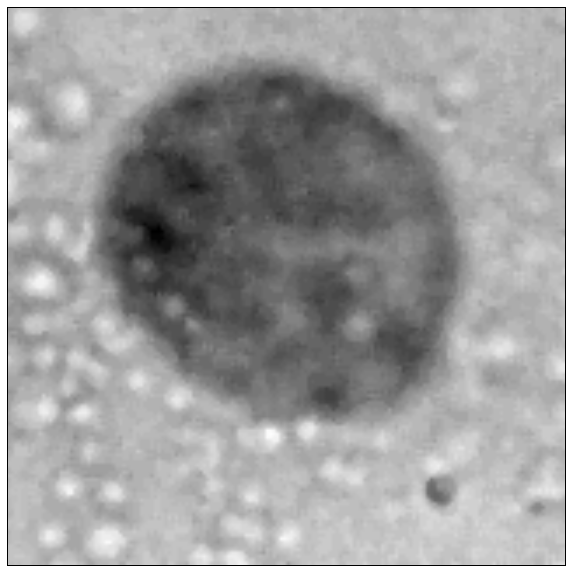
\includegraphics[width=1\linewidth]{Figures/Chapter3/fdim_0_1.png}
	\endminipage\hfill
	\minipage{0.4\textwidth}
	\centering	
	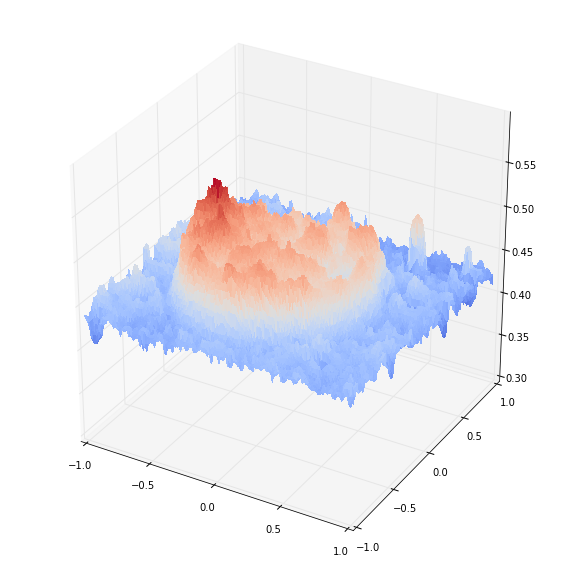
\includegraphics[width=1\linewidth]{Figures/Chapter3/fdim_0_2.png}
	\endminipage\hfill
	\minipage{0.3\textwidth}
	\centering	
	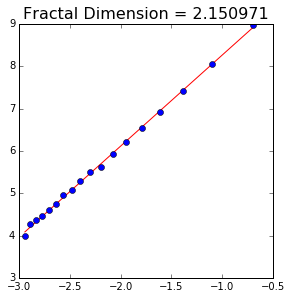
\includegraphics[width=1\linewidth]{Figures/Chapter3/fdim_0_3.png}
	\endminipage\hfill
	\endminipage\hfill
	\minipage{\textwidth}
	\minipage{0.3\textwidth}
	\centering
	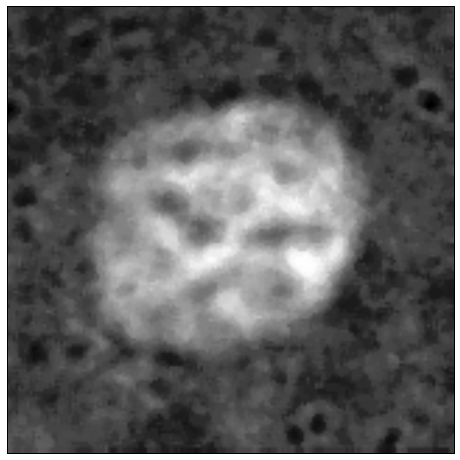
\includegraphics[width=1\linewidth]{Figures/Chapter3/fdim_1_1.png}
	\endminipage\hfill
	\minipage{0.4\textwidth}
	\centering		
	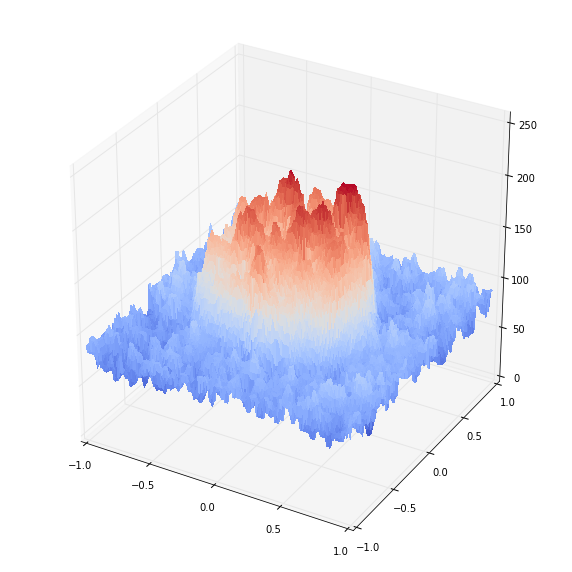
\includegraphics[width=1\linewidth]{Figures/Chapter3/fdim_1_2.png}
	\endminipage\hfill
	\minipage{0.3\textwidth}
	\centering	
	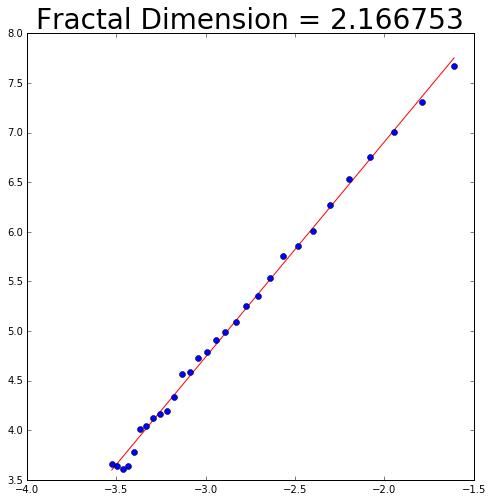
\includegraphics[width=1\linewidth]{Figures/Chapter3/fdim_1_3.png}
	\endminipage\hfill
	\endminipage\hfill
	
	\caption{Фрактальний аналіз зображень.}
	\label{fig:fdim}
\end{figure}

\section{Класифікація пацієнтів}

Слід помітити, що кожному пацієнту ставиться у відповідність набір (вибірка) фрак- тальних характеристик, розмір якої не є сталим. Отже, для порівняння набору характе- ристик різних пацієнтів, треба використовувати міру близькості між вибірками. 

\par
Оскільки міра близькості не є метрикою, вибір методів класифікації є дуже обмеженим. В цій роботі було використано найпростіший спосіб -- метод $k$ найближчих сусідів.

\subsection{Міра близькості та $p \textup{-статистика}$}

Через $H$ позначимо гіпотезу про рівность неперервних функцій розподілу $F_{G}(u)$ і $F_{G'}(u)$ генеральних сукупностей $G$ і $G'$ відповідно. Нехай вибірки $x = \left( x_1, x_2, \dots x_n \right) \in G$ і $x' = \left( x'_1, x'_2, \dots x'_m \right) \in G'$, $x_{(1)} \leq \dots \leq x_{(n)}$, $x_{(1)} \leq \dots \leq x_{(m)}$ -- порядкові статистики. Припустимо що $F_{G}(u) = F_{G'}(u)$. Позначимо через $A_{ij}^{(k)}, k = 1, 2, \dots m$ випадкова подія, яка полягає у тому, що $x'$ потрапляє в інтервал $\left( x_{(i)}, x_{(j)} \right)$, тобто $A_{ij}^{(k)} = \left\{ x'_k \in \left( x_{(i)}, x_{(j)} \right) \right\}$. Як відомо, ймовірність цієї події обчислюється за формулою:
$$P(A_{ij}^{(k)}) = P\left\{ x'_k \in \left( x_{(i)}, x_{(j)} \right) \right\} = p_{ij}^{(n)} = \frac{j-i}{n+1} = \frac{q}{n+1}, \quad q = j-i.$$

Покладемо 
$$ p_{ij}^{(1)} = \frac{ h_{ij}^{(n)}m + \frac{1}{2}g^2 - g\sqrt{h_{ij}^{(n)}(1-h)m + \frac{1}{4}g^2} }{ m+g^2 },$$
$$ p_{ij}^{(2)} = \frac{ h_{ij}^{(n)}m + \frac{1}{2}g^2 + g\sqrt{h_{ij}^{(n)}(1-h)m + \frac{1}{4}g^2} }{ m+g^2 },$$
де $h_{ij}^{(n)}$ -- частота події $A_{ij}^{(k)}$ в $m$ експериментів, величина $g = 3$.

Позначимо через $N$ кількість усіх довірчіх інтервалів $I_{ij}^{(n,m)} = \left( p_{ij}^{(1)}, p_{ij}^{(2)} \right)$ (тобто $N = {n(n-1)}/{2}$) і $L$ -- кількість інтервалів $I_{ij}^{(n,m)}$, які містять ймовірності $p_{ij}^{(n)}$. Покладемо $h^{(n,m)} = \rho(F^{*}, F^{*'}) = \rho(x, x') = {L}/{N}$. Оскільки $h^{(n,m)}$ -- частота випадкової події $B = \left\{ p_{ij}^{(n)} \in I_{ij}^{(n,m)} \right\}$, ймовірність якої дорівнює $p(B) = 1-\beta$, тоді, вважаючи що $h^{n,m}=h^{(n)}$, $m=N$ та $g=3$, отримаємо довірчий інтервал $I^{(n,m} = \left( p^{(1)}, p^{(2)}\right)$ для ймовірності $p(B)$. Статистика $h^{(n)}$ називається $p$-статистикою. Вона також є мірою близькості $\rho(x, x')$ між вибірками $x$ та $x'$ \parencite{bib:pstatistics}.


\subsection{Метод k найближчих сусiдiв. Кросвалідація.}

Використовуючи Метод k найближчих сусiдiв  для класифікації пацієнтів, необхідно зро- бити припущення коректності постулату про компактність:

\begin{conj}
	переважна бiльшiсть об’єктiв, що належать до одного класу, є ближчими один
	до одного, нiж до об’єктiв iншого класу, i лежать в областi з вiдносно простою межею.
\end{conj}

Суть цього методу для класифікації елементу $x$ полягає у тому, що з навчальної вибірки обираємо $k$ найближчих (у розумінні міри близькості) до $x$ елементів (характеристик пацієнтів) та відносимо $x$ до домінантного класу з цих $k$ елементів.

Для пошуку оптимального числа $k$, а також розміру навчальної вибірки $R$ використо- вують метод \textbf{кросвалідації}. Суть цього методу заключається у тому, що для кожного значення $k$ та $R$ випадковим чином підбирається набір даних для навчання.


\section{Результати та спостереження}

Вхідний набір даних для дослідження складається з знімків 6751 інтерфазних ядер букального епітелія, для кожного було зроблено 3 знімки мікроскопу: без фільтру, через жовтий фільтр та через пурпурного фільтру (отже всьго 20253 фотографії), взятого з 130 пацієнтів, з них 68 хворих раком, 29 здорових та 33 хворих іншою хворобою. 

Назвемо групу пацієнтів хворих на рак чи на фіброаденоматоз \enquote{позитивними}, а група здорових пацієнтів \enquote{негативними}. Тоді, за визначенню:

\begin{align*}
\begin{split}
\textup{чутливість} (sensitivity) = \frac{TP}{P}
\\
\textup{специфічність} (specificity) = \frac{TN}{N}
\end{split}
\end{align*}

де \(TP\) (true positive) -- кількість коректно класифікованих позитивних прикладів, \(TN\) (true negative) -- кількість коректно класифікованих негативних прикладів, \(P\) та \(N\) -- кількість позитивних та негативних прикладів у вибірці відповідно.

Нехай \(\Omega = R / N\), де \(R\) -- розмір навчальної вибірки, \(N\) -- розмір усієї вибірки.  Залежність середнього значення (після кросвалідації) чутливості від \(\Omega\) та кількості сусідів, аналі- зуючи червону компоненту зображень:
%-----------------------
%  RED CANCER
%-----------------------
\begin{center}
\begin{tabular}
{cc | c | c | c | c | c | c |}\cline{3-8}
& & \multicolumn{6}{ c| }{Кількість сусідів} \\ \cline{3-8}
& & 6 & 7 & 8 & 9 & 10 & 12 \\ \cline{1-8}

\multicolumn{1}{|c}{\multirow{5}{*}{
		\(\Omega\)
	}}
& \multicolumn{1}{ |c| }{0.5} & 
87.43\% & 81.42\% & 88.86\% & 83.71\% & 87.42\% & 85.43\% 

\\ \cline{2-8}
\multicolumn{1}{ |c  }{} & 
\multicolumn{1}{ |c| }{0.6} & 
83.93\% & 83.93\% & 86.78\% & 83.93\% & 87.14\% & 84.29\%

\\ \cline{2-8}
\multicolumn{1}{ |c  }{} & 
\multicolumn{1}{ |c| }{0.7} & 
85.23\% & 88.10\% & 89.05\% & 90.00\% & 87.62\% & 90.00\%

\\ \cline{2-8}
\multicolumn{1}{ |c  }{} & 
\multicolumn{1}{ |c| }{0.8} & 
87.14\% & 84.29\% & 90.00\% & 89.29\% & 86.43\% & 93.57\%

\\ \cline{2-8}
\multicolumn{1}{ |c  }{} & 
\multicolumn{1}{ |c| }{0.9} & 
82.86\% & 82.86\% & 85.71\% & 84.29\% & 91.42\% & 84.26\%

\\ \cline{1-8}
\end{tabular}
\end{center}



Залежність середнього значення (після кросвалідації) специфічності від \(\Omega\) та кількості сусідів, аналізуючи червону компоненту зображень:
%-----------------------
%  RED FIBRO
%-----------------------
\begin{center}
	\begin{tabular}
		{cc | c | c | c | c | c | c |}\cline{3-8}
		& & \multicolumn{6}{ c| }{Кількість сусідів} \\ \cline{3-8}
		& & 6 & 7 & 8 & 9 & 10 & 12 \\ \cline{1-8}
		
		\multicolumn{1}{|c}{\multirow{5}{*}{
				\(\Omega\)
		}}
		& \multicolumn{1}{ |c| }{0.5} & 
64.00\%	& 74.00\% & 63.33\% & 74.67\% & 62.00\% & 63.33\%
		
		\\ \cline{2-8}
		\multicolumn{1}{ |c  }{} & 
		\multicolumn{1}{ |c| }{0.6} & 
65.83\%	& 70.83\% & 65.33\% & 69.17\% & 64.17\% & 68.33\%
		
		\\ \cline{2-8}
		\multicolumn{1}{ |c  }{} & 
		\multicolumn{1}{ |c| }{0.7} & 
68.89\%	& 72.22\% & 58.89\% & 71.11\% & 73.33\% & 68.89\%
		
		\\ \cline{2-8}
		\multicolumn{1}{ |c  }{} & 
		\multicolumn{1}{ |c| }{0.8} & 
71.67\%	& 65.00\% & 68.33\% & 66.67\% & 73.33\% & 70.00\%
		
		\\ \cline{2-8}
		\multicolumn{1}{ |c  }{} & 
		\multicolumn{1}{ |c| }{0.9} & 
83.33\%	& 83.33\% & 53.33\% & 73.33\% & 66.67\% & 66.67\%
		
		\\ \cline{1-8}
	\end{tabular}
\end{center}


Залежність середнього значення (після кросвалідації) чутливості від \(\Omega\) та кількості сусідів, аналізуючи зелену компоненту зображень:
%-----------------------
%  GREEN CANCER
%-----------------------
\begin{center}
	\begin{tabular}
		{cc | c | c | c | c | c | c |}\cline{3-8}
		& & \multicolumn{6}{ c| }{Кількість сусідів} \\ \cline{3-8}
		& & 6 & 7 & 8 & 9 & 10 & 12 \\ \cline{1-8}
		
		\multicolumn{1}{|c}{\multirow{5}{*}{
				\(\Omega\)
		}}
		& \multicolumn{1}{ |c| }{0.5} & 
		90.86\% & 85.14\% & 	89.71\% & 	86.86\% & 	88.29\% & 	87.71\% 
		
		\\ \cline{2-8}
		\multicolumn{1}{ |c  }{} & 
		\multicolumn{1}{ |c| }{0.6} & 
87.50\% & 83.57\% & 	91.07\% & 	83.57\% & 	90.36\% & 	88.93\% 
		
		\\ \cline{2-8}
		\multicolumn{1}{ |c  }{} & 
		\multicolumn{1}{ |c| }{0.7} & 
81.90\% & 85.71\% & 	90.95\% & 	87.62\% & 	89.04\% & 	83.81\%
		
		\\ \cline{2-8}
		\multicolumn{1}{ |c  }{} & 
		\multicolumn{1}{ |c| }{0.8} & 
81.43\% & 83.57\% & 	88.57\% & 	80.00\% & 	89.29\% & 	91.43\% 
		
		\\ \cline{2-8}
		\multicolumn{1}{ |c  }{} & 
		\multicolumn{1}{ |c| }{0.9} & 
84.29\% & 87.14\% & 	88.57\% & 	87.14\% & 	85.71\% & 	82.86\% 
		
		\\ \cline{1-8}
	\end{tabular}
\end{center}

Залежність середнього значення (після кросвалідації) специфічності від \(\Omega\) та кількості сусідів, аналізуючи зелену компоненту зображень:
%-----------------------
%  GREEN FIBRO
%-----------------------
\begin{center}
	\begin{tabular}
		{cc | c | c | c | c | c | c |}\cline{3-8}
		& & \multicolumn{6}{ c| }{Кількість сусідів} \\ \cline{3-8}
		& & 6 & 7 & 8 & 9 & 10 & 12 \\ \cline{1-8}
		
		\multicolumn{1}{|c}{\multirow{5}{*}{
				\(\Omega\)
		}}
		& \multicolumn{1}{ |c| }{0.5} & 
63.33\% & 	71.33\% & 	67.33\% & 	67.33\% & 	66.67\% & 	60.67\% 
		
		\\ \cline{2-8}
		\multicolumn{1}{ |c  }{} & 
		\multicolumn{1}{ |c| }{0.6} & 
61.67\% & 	69.17\% & 	71.67\% & 	70.00\% & 	67.50\% & 	65.00\% 
		
		\\ \cline{2-8}
		\multicolumn{1}{ |c  }{} & 
		\multicolumn{1}{ |c| }{0.7} & 
71.11\% & 	70.00\% & 	61.11\% & 	77.78\% & 	66.67\% & 	70.00\%  
		
		\\ \cline{2-8}
		\multicolumn{1}{ |c  }{} & 
		\multicolumn{1}{ |c| }{0.8} & 
71.67\% & 	75.00\% & 	70.00\% & 	76.67\% & 	63.33\% & 	71.67\%  
		
		\\ \cline{2-8}
		\multicolumn{1}{ |c  }{} & 
		\multicolumn{1}{ |c| }{0.9} & 
60.00\% & 	63.33\% &  	70.00\% & 	76.67\% & 	73.33\% & 	70.00\%  
		
		\\ \cline{1-8}
	\end{tabular}
\end{center}

Залежність середнього значення (після кросвалідації) чутливості від \(\Omega\) та кількості сусідів, аналізуючи синю компоненту зображень:
%-----------------------
%  BLUE CANCER
%-----------------------
\begin{center}
	\begin{tabular}
		{cc | c | c | c | c | c | c |}\cline{3-8}
		& & \multicolumn{6}{ c| }{Кількість сусідів} \\ \cline{3-8}
		& & 6 & 7 & 8 & 9 & 10 & 12 \\ \cline{1-8}
		
		\multicolumn{1}{|c}{\multirow{5}{*}{
				\(\Omega\)
		}}
		& \multicolumn{1}{ |c| }{0.5} & 
88.86\% &	80.29\% &	86.86\% &	85.71\% &	89.71\% &	86.57\% 

		\\ \cline{2-8}
		\multicolumn{1}{ |c  }{} & 
		\multicolumn{1}{ |c| }{0.6} & 
84.29\% &	84.64\% &	87.14\% &	86.43\% &	90.36\% &	86.43\% 
		
		\\ \cline{2-8}
		\multicolumn{1}{ |c  }{} & 
		\multicolumn{1}{ |c| }{0.7} & 
88.57\% &	85.71\% &	91.90\% &	80.95\% &	90.00\% &	89.53\% 
		
		\\ \cline{2-8}
		\multicolumn{1}{ |c  }{} & 
		\multicolumn{1}{ |c| }{0.8} & 
84.29\% &	80.71\% &	89.29\% &	83.57\% &	90.71\% &	89.29\% 
		
		\\ \cline{2-8}
		\multicolumn{1}{ |c  }{} & 
		\multicolumn{1}{ |c| }{0.9} & 
82.86\% &	81.43\% &	91.43\% &	77.14\% &	92.80\% &	81.43\% 
		
		\\ \cline{1-8}
	\end{tabular}
\end{center}


Залежність середнього значення (після кросвалідації) специфічності від \(\Omega\) та кількості сусідів, аналізуючи синю компоненту зображень:
%-----------------------
%  BLUE CONTROL
%-----------------------
\begin{center}
	\begin{tabular}
		{cc | c | c | c | c | c | c |}\cline{3-8}
		& & \multicolumn{6}{ c| }{Кількість сусідів} \\ \cline{3-8}
		& & 6 & 7 & 8 & 9 & 10 & 12 \\ \cline{1-8}
		
		\multicolumn{1}{|c}{\multirow{5}{*}{
				\(\Omega\)
		}}
		& \multicolumn{1}{ |c| }{0.5} & 
62.67\% &	74.67\% &	66.67\% &	69.33\% &	61.33\% &	62.00\% 
		
		\\ \cline{2-8}
		\multicolumn{1}{ |c  }{} & 
		\multicolumn{1}{ |c| }{0.6} & 
66.67\% &	73.33\% &	65.00\% &	69.17\% &	64.17\% &	67.50\% 
		
		\\ \cline{2-8}
		\multicolumn{1}{ |c  }{} & 
		\multicolumn{1}{ |c| }{0.7} & 
60.00\% &	68.89\% &	62.22\% &	71.11\% &	61.11\% &	60.00\% 
		
		\\ \cline{2-8}
		\multicolumn{1}{ |c  }{} & 
		\multicolumn{1}{ |c| }{0.8} & 
55.00\% &	76.67\% &	65.00\% &	66.67\% &	61.67\% &	68.33\% 
		
		\\ \cline{2-8}
		\multicolumn{1}{ |c  }{} & 
		\multicolumn{1}{ |c| }{0.9} & 
76.67\% &	86.67\% &	70.00\% &	73.33\% &	70.00\% &	53.33\% 
		
		\\ \cline{1-8}
	\end{tabular}
\end{center}


Аналізуючи червону чи зелену компоненту зображень, можна отримати досить гарні результати чутливості та специфічності класифікатора (більші за 80\%). Нажаль, цей метод не дозволяє виявити відмінність між ядрами клітин пацієнтів з фіброаденоматозом та раком молочної залози.
% Chapter Template

\chapter{Глибинне навчання} % Main chapter title

\label{Chapter4} % Change X to a consecutive number; for referencing this chapter elsewhere, use \ref{ChapterX}

Як зазначено у попередньому роздiлi (Роздiл \ref{Chapter3}), фрактальний аналiз текстури iнтерфаз- ного ядра букального епiтелiю i взагалi будь-який алгоритм класифiкацiї, який викорис- товує характеристики текстури та контуру ядра клiтини, добре розпiзнають клас здоро- вих пацiєнтiв вiд пацiєнтiв, хворих раком молочної залози чи фiброаденоматозом, але майже не можуть роздiляти останнi два класи мiж собою. Це пояснюється тим, що цi хвороби викликають дуже схожi гормональнi реакцiї, що призводить до схожих змiн у ядрах ДНК клiтин букального епiтелiю.

Цей роздiл буде присвячено задачi класифiкацiї тiльки класiв хворих раком та фiбро- аденоматозом. За допомогою технiк глибинного машинного навчання, ми намагаємося аналiзувати та використовувати локальнi ознаки та особливостi текстури поверхнi ядра клiтини, якi не можна характеризувати одним числом. 

%----------------------------------------------------------------------------------------
%	SECTION 1
%----------------------------------------------------------------------------------------

\section{Нейронні мережі}

\begin{figure}[b!]
	\minipage{0.5\textwidth}
	\centering	
	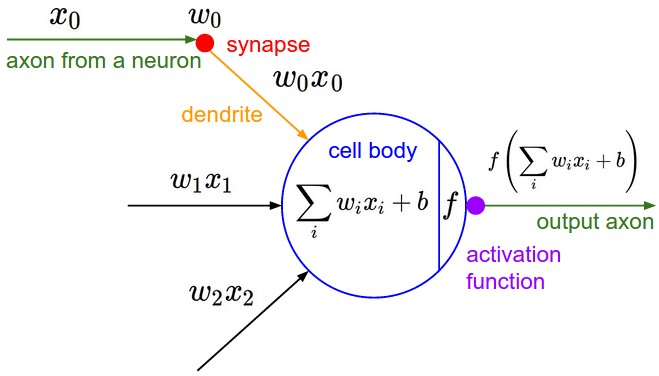
\includegraphics[width=0.90\linewidth]{Figures/Chapter4/neuron_model.jpeg}\\
	(a)
	\endminipage\hfill
	\minipage{0.5\textwidth}
	\centering	
	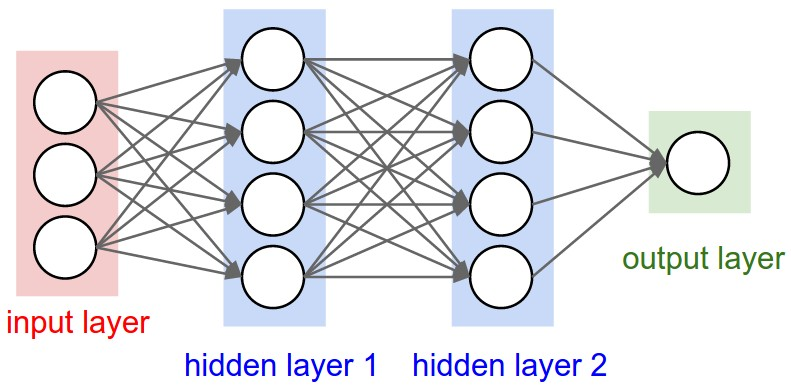
\includegraphics[width=0.90\linewidth]{Figures/Chapter4/neural_net2.jpeg}\\
	(б)
	\endminipage\hfill
	
	\caption{Структура одного нейрону (а) та схема багатошарових перцептронів як граф потоку сигналів (б).}
	\label{fig:neuralnet}
\end{figure}

Штучна нейронна мережа -- це математична модель, яка побудована за принципом функ- цiонування бiологiчних нейронних мереж. Штучнi нейроннi мережi широко використо- вують для задач машинного навчання, розпiзнавання образiв, дискримiнантного аналiзу, кластерування тощо. 

Нейронну мережу можна iнтерпретувати як граф. У підручнику \citep{book:haykin}, нейроннi мережi описуються як граф потоку сигналу (signal-flow graph), де кожен нейрон (або вершина у графi) є окремою одиницею обчислення. Схема одного штучного нейрону зображена на (Мал. \ref{fig:neuralnet} (а)).

Кожен нейрон мережi має справу лише з сигналами, якi вiн перiодично отримує, i сигналами, якi вiн перiодично надсилає iншим нейронам. i тим не менш, будучи з'єдна- ними в достатньо велику мережу з керованою взаємодiєю, такi простi нейрони разом здатнi моделювати складнi функцiї, виявляти складнi залежностi мiж вхiдними й вихiд- ними даними, а також здiйснювати узагальнення.


\subsection{Багатошаровий перцептрон}

Штучний багатошаровий перцептрон -- це така архiтектура нейронних мереж, у якiй групи нейронiв формують \enquote{шари}, в яких кожний нейрон з одного шару зв'язана з усiма нейронами сусiднього шару. Отже, сигнали на вихiд одного шару нейронiв є сигналами на вхiд нейронiв наступного шару. На (Мал. \ref{fig:neuralnet} (б)) зображено схему багатошарового перцептрону. Такi шари нейронiв також називають \enquote{повнiстю зв'язаними} (Fully connected layers).

\subsection{Функція активації ReLU}

У цiй роботi було використано функцiю зрiзаних лiнiйних вузлiв, або ReLU, для активацiї нейронiв замiсть сигмоїдальних функцiй чи гiперболiчного тангенсу. Функцiя активацiї ReLU (Rectified Linear Unit), яка задається наступним чином:

\begin{equation*}
f(x) = \max(0, x)
\end{equation*}

має багато переваг над сигмоїдальними функцiями чи гiперболiчним тангенсом при використаннi в якостi функцiї активацiї:

\begin{itemize}
	\item В роботi \parencite{nn:krizhevsky_imagenet}, було доведено що така функцiя активацiї може прискорити збiжнiсть спуску за градiєнтом до 6 разiв у порiвняннi з сигмоїдальними функцiями чи гiперболiчними тангенсами.
	
	\item Сигмоїдальнi функцiї та гiперболiчнi тангенси використовують складнi операцiї, такi як зведення у степiнь.
\end{itemize}

Детальний аналiз переваг та недолiкiв цiєї функцiї, а також позбавлення недолiкiв за допомогою модифiкованої версiї \enquote{Leaky ReLU}, описаний в роботi \parencite{nn:kaiming}.


\subsection{Згорткові нейронні мережі}

Згортковi нейроннi мережi -- це мережi, якi мiстять згортковi шари нейронiв, уперше запропонований \parencite{nn:lecun_cnn}. Згортковий шар нейронiв мiстить фiльтри -- набiр ваг. При подачi даних на вхiд, вихiдний сигнал обчислюється як згортка фiльтру з локальним регiоном зображення. На (Мал. \ref{fig:convonet} (а)) показано схему першого згорткового шару, де кожен нейрон локально зв'язаний з пiкселями зображення та \enquote{бачить} усi канали. Кiлькiсть шарiв нейронiв у згортковому шару (зображено кружечками) дорiвнює кiлькостi фiльтрiв згорткового шару, тобто для рiзних шарiв нейронiв використовується рiзнi фiльтри.

Згортковi нейроннi шари використовують для виявлення локальних особливостей зобра- ження. Цi шари також дозволяють мережi бути бiльш стiйкою до трансляцiї, тобто надають деяку iнварiантнiсть. Тому, будемо використовувати згортковi шари для побу- дови класифiкатора мiж хворими раком та фiброаденоматозом.

Разом iз згортковими нейронними шарами також будемо використовувати пiдвибiрковi шари (pooling layers), якi значно зменшують обсяг вхiдних даних на наступнi шари мережi.

\begin{figure}[t!]
	\minipage{0.4\textwidth}
	\centering	
	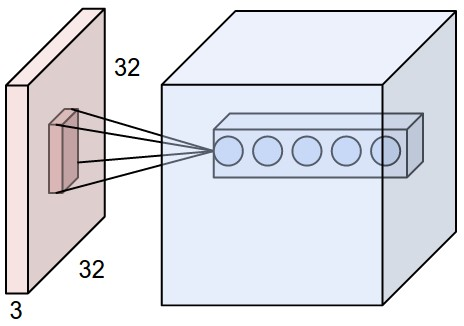
\includegraphics[width=0.90\linewidth]{Figures/Chapter4/depthcol.jpeg}\\
	(a)
	\endminipage\hfill
	\minipage{0.6\textwidth}
	\centering	
	\includegraphics[width=0.90\linewidth]{Figures/Chapter4/cnn.jpeg}\\
	(б)
	\endminipage\hfill
	
	\caption{На (а) схематично зображено згортковий шар. На (б) зображено схему згорткової мережі.}
	\label{fig:convonet}
\end{figure}

\subsection{Алгоритм RMSProp}

Пiсля обчислення градiєнтiв за допомогою алгоритму зворотного поширення помилок (backpropagation), цi градiєнти використовуються для оновлення параметрiв (ваг) ней- ронної мережi. Зазначимо, що оптимiзацiя алгоритму оновлення нейронних мереж є на момент написання цiєї роботи дуже активною сферою дослiджень.

Алгоритм RMSProp \citep{nn:rmsprop} є дуже ефективним, але ще не опублiкований метод адаптивного оновлювання параметрiв. Вiн налаштовує та регулює алгоритм Adagrad \parencite{nn:adagrad} таким чином щоб зменшити рiзкiсть монотонного зменшення швидкостi навчання. На вiдмiну вiд Adagrad, цей алгоритм використовує так званi \enquote{ковзаючi} середньоквадратичнi значення градiєнтiв:

\begin{equation*}
cache = decay\_rate \cdot cache + (1 - decay\_rate) \cdot dx^2
\end{equation*}
\begin{equation*}
x = x - \frac{learning\_rate \cdot dx}{\sqrt{cache} + eps}
\end{equation*}

де \(decay\_rate\) це гiперпараметр, якому зазвичай присвоюють значення з множини чисел \(\{0.9, 0.99, 0.999\}\). Отже, метод RMSProp також модулює швидкiсть навчання кожного параметру з урахуванням величин його градiєнтiв, що має вигiдний ефект вирiвнювання. Але, на вiдмiну вiд Adagrad, величини оновлень не зменшуються монотонно.

У цiй роботi використовується саме алгоритм RMSProp. На практицi бiльш стандартним методом для оновлення параметрiв є алгоритм Adam (adaptive moment estimation) \parencite{nn:adam}, який дуже схожий на RMSProp та у деяких випадках є трохи ефективнiшим нiж RMSProp, але цей алгоритм є бiльш громiздким та потребує трохи бiльше часу для обчислень. Повний алгоритм Adam також включає механiзм корекцiї змiщень. Альтернативою RMSProp та Adam є також комбiнацiя алгоритмiв SGD та Nesterov Momentum.

\subsection{Регуляризація нейронної мережі}

\begin{figure}[t]
	\centering
	\minipage{0.7\textwidth}
	\minipage{0.5\textwidth}
	\centering	
	\includegraphics[width=0.8\linewidth]{Figures/Chapter4/dropout1.png}
	\\ (а) До Dropout
	\endminipage\hfill
	\minipage{0.5\textwidth}
	\centering	
	\includegraphics[width=0.8\linewidth]{Figures/Chapter4/dropout2.png}
	\\ (б) Після Dropout
	\endminipage\hfill
	\endminipage\hfill
	
	\caption{Візуалізація методу Dropout з ймовірністю \(p = 0.5\).}
	\label{fig:dropout}
\end{figure}

Процес регуляризацiї нейронної мережi -- це процес уникнення перенавчання (overfitting) мережi. iснує кiлька способiв контролювання тренування нейронної мережi, щоб максимальним чином уникнути перенавчання.

У цiй роботi використовується метод Dropout -- простий та дуже ефективний метод регуляризацiї, запропонований \parencite{nn:dropout}. При тренуваннi, кожен нейрон є активним за ймовiр- нiстю \(p\) (що є гiперпараметром мережi).

На (Мал. \ref{fig:dropout}) схематично зображено принцип роботи методу Dropout. На практицi також часто використовують алгоритми \(L1\)- та \(L2\)- регуляризацiї нейронних мереж \citep{nn:l1l2regularization}, разом з методом Dropout.

\subsection{Функція втрат. Перехрестна ентропія.}

Вибiр функцiї втрат є одним з найважливiших крокiв при побудовi моделi класифiкатора. Вдало обрана функцiя втрат може значно покращити результат та швидкiсть тренування класифiкатора.

На практицi при тренуваннi класифiкаторiв на основi нейронних мереж найчастiше використовують перехресну ентропiю (categorical crossentropy):
\begin{equation*}
L_i = -\log\left(\frac{e^{f_{y_i}}}{ \sum_j e^{f_j} }\right)
\end{equation*}

яка для випадку задач класифiкацiї дає кращi результати, нiж середньоквадратична функцiя втрат (mean square error) та функцiя помилки класифiкацiї (classification error). У цiй роботi використовується саме ця функцiя оцiнювання втрат. Слiд також зазначити, що при тренуваннi моделi та при класифiкацiї чи обчисленнi можна використовувати рiзнi оцiнки втрат.

%----------------------------------------------------------------------------------------
%	SECTION 2
%----------------------------------------------------------------------------------------

\section{Класифікація за допомогою нейронних мереж}


\subsection{Прирощення даних}

Як вказано у роздiлi \ref{Chapter1}, для дослiдження маємо тiльки набiр даних який мiстить 3403 зображень iнтерфазних ядер букального епiтелiю, взятих з 68 пацiєнтiв хворих раком молочної залози, та 1741 зображень ядер взятих з 33 пацiєнтiв хворих фiброаденоматозом. Така кiлькiсть є дуже малою для тренування глибоких згорткових нейронних мереж. Отже, будемо штучно збiльшувати кiлькiсть даних для тренування.  

При подачi в нейронну мережу випадковим чином зробимо декiлька з наступних пере- творень над зображеннями:
\begin{itemize}
\item Перевернути зображення вiдносно горизонтальної осi
\item Перевернути зображення вiдносно вертикальної осi
\item Повернути зображення на випадковий кут вiд \(0\) до \(2\pi\), при чому пiкселi, що до перетворення знаходилися за межами входу, присвоюються значенню сусiднiх пiк- селiв.
\end{itemize}

\begin{figure}[t!]
	\minipage{0.2\textwidth}
	\centering
	\includegraphics[width=0.97\linewidth]{Figures/Chapter4/aug_0.png}	
	\endminipage\hfill
	\minipage{0.2\textwidth}
	\centering	
	\includegraphics[width=0.97\linewidth]{Figures/Chapter4/aug_1.png}
	\endminipage\hfill
	\minipage{0.2\textwidth}
	\centering	
	\includegraphics[width=0.97\linewidth]{Figures/Chapter4/aug_2.png}
	\endminipage\hfill
	\minipage{0.2\textwidth}
	\centering	
	\includegraphics[width=0.97\linewidth]{Figures/Chapter4/aug_3.png}
	\endminipage\hfill
	\minipage{0.2\textwidth}
	\centering	
	\includegraphics[width=0.97\linewidth]{Figures/Chapter4/aug_4.png}
	\endminipage\hfill	
	
	\caption{Прирощення даних на прикладі одного зображення.}
	\label{fig:data_augmentation}
\end{figure}


\subsection{Проблема незбалансованості вибiрки для тренування}

Для тренування було обрано випадковим чином \(80\%\) вiд всього набору даних. Це стано- вить 1392 зображень взятих з 33 пацiєнтiв хворих фiброаденоматозом та 2722 зображень з 68 пацiєнтiв хворих раком молочної залози. Отже, в набiр даних для валiдацiї входять iншi зображення ядер букального епiтелiю тих самих пацiєнтiв. Маємо незбалансованiсть вибiрки для тренування, де кiлькiсть даних з одного класу (з класу хворих раком) майже вдвiчi перевищує кiлькiсть даних з iншого класу (хворих фiброаденоматозом). 

Незбалансованiсть набору даних для тренування може значно негативно вплинути на навчання класифiкатора \citep{nn:imbalance2}. Слiд зазначити, що набiр даних для валiдацiї теж є незба- лансованим. Так, пiсля тренування моделi на незбалансованiй вибiрцi, автором цiєї робо- ти було отримано класифiкатор, точнiсть розпiзнавання якого на обох наборах даних для тренування i тестування становила бiльш нiж 65\%. Подальший аналiз результатiв виявив, що отримана модель має чутливiсть, близьку до 100\% та специфiчнiсть, близьку до 0\%, тобто модель у бiльшостi випадкiв просто класифiкувала зображення як \enquote{нале- жить хворого раком}. Отже, необхiдно знайти спосiб боротьби з проблемою незбалансо- ваностi набору даних для тренування.

Існує багато методiв для боротьби з цiєю проблемою. Найбiльш поширеними на практицi є методи змiни об'єму даних (subsampling methods) та методи навчання з вагами (cost-sensitive methods) \citep{nn:imbalance}, де рiзним класам присвоюється деяке значення \enquote{критичностi} помилки. Було вирiшено використовувати перший метод.

Отже, пiсля змiни об'єму даних, кiлькiсть зображень для тренування становить 1392 з хворих фiброаденоматозом та 1632 з хворих раком молочної залози, а кiлькiсть зобра- жень для валiдацiї становить 349 зображень з хворих фiброаденоматозом та 1771 зобра- жень з хворих раком молочної залози.

\subsection{Архітектура мережі}

Для зручного опису архiтектури мереж, використаємо наступнi позначення:

\begin{itemize}
	\item Позначимо повністю зв'язані шари нейронів (fully-connected layers) як \(xFC\), де \(x\) -- кількість нейронів шару. Наприклад, якщо повністю зв'язаний шар має 128 нейронів, то позначаємо \(128FC\).
	
	\item Згорткові нейронні шари (convolutional layers), де фільтри шару мають розміри \(x \times x\), позначимо як \(yCONVx\), де \(y\) -- кількість фільтрів. Наприклад, \(64CONV3\).
	
	\item Підвибіркові шари (max-pooling layers) позначимо як \(MPx\), де \(x\) -- розмір ядра фільтру. Наприклад, \(MP2\).
	
	\item Вхідні (input) та вихідні (output) дані позначимо як \(I\) та \(O\) відповідно.
	
	\item Домовимось, що сигнал протікає з шару, що знаходиться лівіше у записі, до шару, що знаходиться правіше. Сусідні шари нейронів з'єднуємо символом \enquote{\(\rightarrow\)}. Повна архітектура мережі так: \(I \rightarrow 32CONV3 \rightarrow MP2 \rightarrow FC16 \rightarrow O\).
\end{itemize}

Автором було розглянуто багато рiзних архiтектур нейронної мережi. Окрiм простих вiдносно неглибоких архiтектур згорткової нейронної мережi, якi схожi на AlexNet, також були розглянутi мережi, подiбнi до VGG \cite{nn:vgg}.

\bigskip
\begin{itemize}
	\label{arch}
	
	\item[ARCH-0]
	\(I \rightarrow
	32CONV3 \rightarrow
	MP2 \rightarrow
	32CONV3 \rightarrow
	MP2 \rightarrow
	64CONV5 \rightarrow
	MP2 \rightarrow
	FC32 \rightarrow
	FC32 \rightarrow
	O \)
	
	\item[ARCH-1]
	\(I \rightarrow
	32CONV3 \rightarrow
	MP2 \rightarrow
	48CONV3 \rightarrow
	MP2 \rightarrow
	64CONV3 \rightarrow
	MP2 \rightarrow
	72CONV3 \\ \rightarrow 
	MP2 \rightarrow
	FC64 \rightarrow
	FC64 \rightarrow
	O \)
	
	\item[ARCH-2]
	\(I \rightarrow
	64CONV5 \rightarrow
	48CONV3 \rightarrow
	MP2 \rightarrow
	FC32 \rightarrow
	FC16 \rightarrow
	O \)
	
	\item[ARCH-3]
	\(I \rightarrow
	64CONV3 \rightarrow
	MP2 \rightarrow
	64CONV3 \rightarrow
	MP2 \rightarrow
	96CONV3 \rightarrow
	MP2 \rightarrow
	96CONV3 \\ \rightarrow
	MP2 \rightarrow
	FC48 \rightarrow
	FC48 \rightarrow
	O \)
		
	\item[VGG-9]
	\(I \rightarrow
	32CONV3 \rightarrow
	32CONV3 \rightarrow
	MP2 \rightarrow
	48CONV3 \rightarrow
	48CONV3 \rightarrow
	MP2 \rightarrow
	64CONV5 \rightarrow
	64CONV5 \rightarrow
	MP2 \rightarrow
	FC32 \rightarrow
	FC32 \rightarrow
	O \)
	
	\item[VGG-11]
	\(I \rightarrow 
	48CONV3 \rightarrow 
	48CONV3 \rightarrow 
	MP2 \rightarrow 
	64CONV3 \rightarrow 
	64CONV3 \rightarrow 
	MP2 \rightarrow 
	72CONV3 \rightarrow 
	72CONV3 \rightarrow 
	MP2 \rightarrow 
	96CONV3 \rightarrow 
	96CONV3 \rightarrow 
	MP2 \rightarrow
	FC96 \rightarrow
	FC96 \rightarrow
	O \)
	
	\item[VGG-13]
	\(I \rightarrow 
	32CONV3 \rightarrow 
	32CONV3 \rightarrow 
	MP2 \rightarrow 
	64CONV3 \rightarrow 
	64CONV3 \rightarrow 
	MP2 \rightarrow 
	128CONV3 \rightarrow 
	128CONV3 \rightarrow 
	MP2 \rightarrow 
	256CONV3 \rightarrow 
	256CONV3 \rightarrow 
	MP2 \rightarrow
	256CONV3 \rightarrow 
	256CONV3 \rightarrow 
	MP2 \rightarrow
	FC128 \rightarrow
	FC128 \rightarrow
	O \)
\end{itemize}

Для кожного шару нейронiв цих архiтектур було використано ReLU в якостi функцiї активацiї, а для кiнцевого шару \(O\) з одного нейрону (якщо на виходi 0 то зображення класифiкується як належним до хворого раком молочної залози, а якщо 1 -- то класифi- кується як належним до хворого фiброаденоматозом) було використано функцiю актива- цiї SoftMax. З метою регулювання, для кожного повнiстю зв'язаного шару було викорис- тано алгоритм Dropout. В якостi алгоритму задання швидкостi навчання (тобто оновлення параметрiв) використовується RMSProp.


\subsection{Тренування мереж та результати}

\begin{figure}[t!]
	\includegraphics[width=\linewidth]{Figures/Chapter4/best_model.png}
	\caption{Архітектура найкращої мережі.}
	\label{fig:best_model}
\end{figure}

Слiд зазначити, що вибiр архiтектури обмежувався потужнiстю доступних автору обчис- лювальних ресурсiв. У розпорядженнi автора на момент дослiдження був комп'ютер з процесором Intel Core i7, комп'ютер з процесором Intel Core i3, а також вiдеокарта Nvidia Geforce GT 520M. Отже, використання бiльш глибоких нейронних мереж, або мереж з бiльшою кiлькiстю вiльних параметрiв, не було можливим.

Кожна з перерахованих вище мереж тренувалася по декiлька (для ARCH-0 -- декiлька десяткiв) разiв, кожен раз нейронна мережа iнiцiалiзувалася випадковим набором ваг (параметрiв) та навчалася протягом 300 епох. Кожна епоха -- це цикл, в якому нейронна мережа навчається на даних, якi по обсягу дорiвнюють об'єму тренувальної вибiрки. Неповторнiсть вхiдних даних для тренування гарантує алгоритм прирощення даних. Також були використанi рiзнi значення для Dropout, вiд \(0.2\) до \(0.5\).

Сумарно навчання вищеописаних мереж проводилось протягом трьох тижнiв. Найбiльш повiльними для навчання є моделi VGG-9, VGG-11 та VGG-13. У середньому на навчання цих моделей протягом 300 епох пiшло бiльш нiж 48 годин процесорного часу.

Найбiльш вдалою є архiтектура ARCH-0, яка схематично зображена на (Мал. \ref{fig:best_model}). Нижче у таблицi приведенi найкращi результати класифiкацiї окремого зображення iнтерфаз- ного ядра клiтини букального епiтелiю цих мереж.

\bigskip
\begin{center}
\begin{tabular}
{| m{3cm} || m{3cm} | m{3cm} | m{3cm} |}
\hline
Архітектура & Чутливість & Специфічність & Точність \\ \hline \hline
ARCH-0 & 59.17\%  & 67.33\%  & 62.93\%  \\ \hline
ARCH-1 & 55.74\%  & 57.59\%  & 56.60\%  \\ \hline
ARCH-2 & 67.24\%  & 53.58\%  & 60.95\%  \\ \hline
ARCH-3 & 56.72\%  & 58.45\%  & 57.52\%  \\ \hline
VGG-9  & 55.25\%  & 59.89\%  & 57.39\%  \\ \hline
VGG-11 & 58.43\%  & 58.45\%  & 58.44\%  \\ \hline
VGG-13 & 56.23\%  & 55.59\%  & 55.94\%  \\ \hline
\end{tabular}
\end{center}
\bigskip

Найкращi результати за точнiстю дає мережа ARCH-0. Надалi будемо детальнiше аналi- зувати її результати та намагатися побудувати класифiкатор з кращими результатами на основi цiєї моделi.

Можна розглядати кожне зображення ядра клітини певного пацієнта не окремо, а у сукупності з іншими зображеннями клітин цього пацієнта, тобто класифікувати не належ- ність окремого ядра букального епітелію до класу хвороби, а належність самого пацієнта до цих класів. Наприклад, якщо більшість зображень ядер клітин цього пацієнта класи- фікується належними до класу \enquote{хворі раком}, то віднесемо цього пацієнта до класу \enquote{хворий раком} (аналогічно з фіброаденоматозом). Тоді отримаємо наступні результати:


\begin{center}
	\begin{tabular}
		{| m{3cm} || m{3cm} | m{3cm} | m{3cm} |}
		\hline
		Архітектура & Чутливість & Специфічність & Точність \\ \hline \hline
		ARCH-0 & 58.82\%  & 69.70\%  & 62.38\%  \\ \hline
	\end{tabular}
\end{center}

що незначно вiдрiзняються вiд результатiв, отриманих при класифiкацiї окремих клiтин.

\subsection{Аналіз результатів}

Помiтимо, що мережа з вiдносно простою архiтектурою ARCH-0 дає кращi результати нiж VGG-подiбнi мережi. Це можна пояснити тим, що VGG-подiбнi глибокi архiтектури мiстять у декiлька десяткiв разiв бiльше вiльних параметрiв, а отже, потребують бiльше нiж 300 епох для навчання. При тренуваннi моделi VGG-11, наприклад, спостерiгалося дуже вiльне спадання значення функцiї втрат. Це свiдчить про те, що, можливо, треба було обирати iншi гiперпараметри для мережi, такi як \(learning\_ rate\) для алгоритму RMSProp, або використовувати менший \(batch\_size\) (обсяг даних при тренуваннi, пiсля якого обчислюється градiєнт та виконується одне оновлення параметрiв).

\section{Підвищення якості розпізнавання}

Надалi будемо будувати бiльш точний класифiкатор на основi отриманої моделi нейрон- ної мережi ARCH-0. Щоб переконатися у тому, що ця модель дiйсно генералiзується на невiдомi данi (тi, якi не було використано при тренуваннi), розглянемо розподiл вихiдних значень мережi для обох наборiв: тренування та валiдацiї, що показанi на (Мал. \ref{fig:train_distribution}). Можна побачити, що отримана мережа добре генералiзується на вибiрцi для валiдацiї.

\begin{figure}[t!]
	\minipage{0.5\textwidth}
	\centering	
	\includegraphics[width=0.95\linewidth]{Figures/Chapter4/train_dist_cancer.png}\\
	(a)
	\endminipage\hfill
	\minipage{0.5\textwidth}
	\centering	
	\includegraphics[width=0.95\linewidth]{Figures/Chapter4/train_dist_fibro.png}\\
	(б)
	\endminipage\hfill
	\\	
	\minipage{0.5\textwidth}
	\centering	
	\includegraphics[width=0.95\linewidth]{Figures/Chapter4/test_dist_cancer.png}\\
	(в)
	\endminipage\hfill
	\minipage{0.5\textwidth}
	\centering	
	\includegraphics[width=0.95\linewidth]{Figures/Chapter4/test_dist_fibro.png}\\
	(г)
	\endminipage\hfill
	
	\caption{Розподіл значення виходу мережі на зображеннях ядер с вибірки для тренування, що належить пацієнтам хворі на рак (а) та на фіброаденоматоз (б). На (в) та (г) зображено розподіл виходу мережі на зображеннях ядер з вибірки для тестування що належить пацієнтам хворі на рак та фіброаденоматоз відповідно.}
	\label{fig:train_distribution}
\end{figure}

Отже, припускаючи, що розподiл вихiдних значень мережi для пацiєнтiв з однаковою хворобою (рак молочної залози чи фiброаденоматоз) буде також приблизно однаковими, замiсть простого пiдходу, що описаний у попередньому пiдроздiлi, можна розглядати нейронну мережу не як бiнарний класифiкатор, а як генератор ознак, тобто кожному зображенню ставити у вiдповiднiсть деяке число (ознаку). Отже, до кожного пацiєнта (набору зображень) можна застосовувати статистичнi тести.



\subsection{Гибрідний класифікатор}

В якостi критерiю еквiвалентностi генеральних сукупностей було використано критерiй Колмогорова-Смiрнова, що є одним з найефективнiших непараметричних критерiїв для порiвняння вибiрок. Альтернативно можна використовувати \(p\)-статистику, що детально описана у попередньому роздiлi. 

Нехай \(can\_trainX\) -- сукупнiсть зображень iнтерфазних ядер букального епiтелiю у вибiрцi для тренування, взятих з пацiєнтiв хворих раком, а \(fib\_trainX\) -- сукупнiсть зображень ядер у вибiрцi для тренування взятих з пацiєнтiв хворих фiброаденоматозом.  

При класифiкацiї деякого пацiєнта \(P = \{X^1, X^2, \dots X_n\} \) обчислюється: 
\begin{equation*}
can\_train = \textup{ARCH-0}(can\_trainX) = \{\textup{ARCH-0}(X)\,\, \forall X \in can\_trainX\}
\end{equation*}
\begin{equation*}
fib\_train = \textup{ARCH-0}(fib\_trainX) = \{\textup{ARCH-0}(X)\,\, \forall X \in fib\_trainX\}
\end{equation*}
\begin{equation*}
M = \textup{ARCH-0}(P) = \{\textup{ARCH-0}(X^i)\,\, \forall i \in 1 \dots n\}
\end{equation*}

де \(\textup{ARCH-0}(X)\) -- значення виходу нейронної мережi пiсля обробки зображення \(X\). Потiм, обчислюється \(p\)-значення статистики Колмогорова-Смiрнова спочатку для \(can\_train\) та \(M\), а потiм для \(fib\_train\) та \(M\). Цi значення використаємо як показних схожостi цих вибiрок.

\subsection{Аналіз результатів}

У таблиці показано результати класифікації пацієнтів як сукупність ядер клітин, отрима- ні за підходом, що описаний вище.

\begin{center}
	\begin{tabular}
		{| m{3cm} || m{3cm} | m{3cm} | m{3cm} |}
		\hline
		Архітектура & Чутливість & Специфічність & Точність \\ \hline \hline
		ARCH-0 & 70.59\%  & 63.64\%  & 68.32\%  \\ \hline
	\end{tabular}
\end{center}

Слiд зазначити, що в нашому випадку у зв'язку зi змiною обсягу даних для навчання спостерiгається значна незбалансованiсть класiв у наборi даних для валiдацiї, а саме: 1771 зображень ядер, взятих з 68 пацiєнтiв хворих раком, та 349 -- з хворих фiброадено- матозом. Отже, кожний пацiєнт, хворий раком, має у середньому 26 зображень клiтин ядер у наборi даних для валiдацiї, та в той же час кожен пацiєнт, що хворий фiброадено- матозом, має у середньому 10 зображень клiтин ядер у вибiрцi для валiдацiї. Саме тому спостерiгається така рiзниця мiж чутливiстю та специфiчнiстю моделi пiсля валiдацiї. Можна висловити припущення, що маючи достатню кiлькiсть зображень для класифi- кацiї конкретного пацiєнта, можна досягти чутливостi та специфiчностi бiльшi за 71\%.

Перегрупуємо данi за пацiєнтами, залишаючи мережу ARCH-0 тою самою. Отже, для тестування маємо окремих пацiєнтiв, для кожного з яких доступно по 50 клiтин для валiдацiї. Припускаючи, що розподiл вихiдних значень мережi ARCH-0 однаковий для всiх пацiєнтiв однакової категорiї (з однаковою хворобою) та використовуючи метод, описаний вище, отримуємо наступнi результати (чутливiсть, специфiчнiсть та точнiсть у середньому пiсля кросвалiдацiї):

\begin{center}
	\begin{tabular}
		{| m{3cm} || m{3cm} | m{3cm} | m{3cm} |}
		\hline
		Архітектура & Чутливість & Специфічність & Точність \\ \hline \hline
		ARCH-0 & 71.32\%  & 78.95\%  & 73.81\%  \\ \hline
	\end{tabular}
\end{center}

Отже, пiдхiд з використанням згорткових нейронних мереж та статистичних методiв має дуже перспективнi результати для подальшого дослiдження. 
% Chapter Template

\chapter{Висновок} % Main chapter title

\label{Chapter5} % Change X to a consecutive number; for referencing this chapter elsewhere, use \ref{ChapterX}

%----------------------------------------------------------------------------------------
%	SECTION 1
%----------------------------------------------------------------------------------------

У цій роботі було використано методи комп'ютерного зору для сегментації зображень інтерфазних ядер букального епітелію, досліджено взаємозв'язок між характеристиками зображень цих ядер та наявністю пухлин в молочній залозі пацієнтів за допомогою фрактальних показників і статистичних методів та запропоновано метод класифікації пацієнтів хворих на рак та на фіброаденоматоз за цими зображеннями на основі новітніх методів машинного навчання. Використаний метод сегментації зображень виявився дуже точним для цієї конкретно поставленої задачі, а запропонований швидкий алгоритм для фільтру зображень на основі еліпсоїдів Петуніна є не менш ефективним за часом, ніж звичайний алгоритм для медіанної фільтрації. Отримано дужі точні результати розпізнавання здорових пацієнтів від хворих раком молочної залози чи фіброаденома- тозом. Запропонований метод класифікації пацієнтів хворих на рак та на фіброаденома- тоз за допомогою глибинного навчання та статистичних критеріїв дає дуже перспективні результати. 



\section{Поради для подальших досліджень}

Відмінність між локальними ознаками на зображеннях інтерфазних ядер букального епітелію у пацієнтів з раком молочної залози та фіброаденоматозом, на відміну від зв'язку між характеристиками цих ядер та наявністю пухлин в молочной залозі пацієнтів \citep{bib:the_beginning}, є ще мало дослідженою. Подальші дослідження у цьому напрямку є дуже перспек- тивними. Автор цієї роботи робить припущення, що використовуючи більш ефективні методи глибинного навчання, можна отримати результати, що будуть набагато точні- шими за отримані.


Як зазначено у розділі \ref{Chapter4}, використання відносно неглибоких архітектур у цій роботі зумовлене відсутністю доступу до більш потужних обчислювальних ресурсів на момент написання цієї роботи. Більш того, новітні дослідження в області глибинного навчання пропонують методи для значного прискорення процесу тренування згорткової нейронної мережі. Так, наприклад, у роботах \citep{nn:perforated} та \citep{nn:acceleration} пропонуються методи прискорення нейрон- них мереж при обчисленнях та навчанні у декілька разів без значної втрати точності. Такі прискорення є доречними при використанні для таких глибоких архітектур як VGG-16 \citep{nn:vgg}, AlexNet \citep{nn:krizhevsky_imagenet} та NIN \citep{nn:nin}. Рекомендується також обрати більш оптимальні гіперпараметри, наприклад, початкові ваги чи коефіцієнти для RMSProp чи інших алго- ритмів оновлення параметрів, а також використовувати методи навчання з вагами \citep{nn:imbalance} чи інші методи для боротьби з проблемою незбалансованості вибірки для тренування. Крім цього, щоб отримати більш точні результати, необхідний більший обсяг даних з кращою якістю для аналізу. 

%----------------------------------------------------------------------------------------
%	THESIS CONTENT - APPENDICES
%----------------------------------------------------------------------------------------

\appendix % Cue to tell LaTeX that the following "chapters" are Appendices

% Include the appendices of the thesis as separate files from the Appendices folder
% Uncomment the lines as you write the Appendices

% Appendix A

\chapter{Програмний пакет} % Main appendix title

\label{AppendixA} % For referencing this appendix elsewhere, use \ref{AppendixA}

В процесі виконання цієї роботи для кожного розділу було створено комплекс програм. Детальний опис, інструкцію щодо встановлення та код програм можна знайти за посилан- ням на git-репозиторій: \href{https://github.com/chankhavu/CancerDetection}{https://github.com/chankhavu/CancerDetection}.
%\include{Appendices/AppendixB}
%\include{Appendices/AppendixC}

%----------------------------------------------------------------------------------------
%	BIBLIOGRAPHY
%----------------------------------------------------------------------------------------

\printbibliography[heading=bibintoc]


%----------------------------------------------------------------------------------------

\end{document}  
